% Tratto da grfguide.[ps|pdf]:
%
%\graphicspath{<dir-list>}
%    This optional declaration may be used to specify a list of directories in which to search
%    for graphics files. The format is the same as for the LATEX 2e primitive \input@path.
%    A list of directories, each in a {} group (even if there is only one in the list). For example:
%    \graphicspath{{eps/}{tiff/}}
%    would cause the system to look in the subdirectories eps and tiff of the current directory.
%
%\graphicspath{{FIGS/}}
%
% E` preferibile fare come segue, perche' in questo modo ad es. anche i .tex
% possono essere messi in altre directory e inclusi senza indicarne il percorso.
\makeatletter
\let\input@path=\@undefined
\def\input@path{{FIGS/}}
\makeatother

\ifx\pdfoutput\undefined % We are not running pdftex
\documentclass[12pt,a4paper]{report}




\usepackage[dvips]{graphicx,color}


\usepackage{caption,subcaption}% http://ctan.org/pkg/{caption,subcaption}
% \usepackage{psfig}
% \usepackage{epsfig}
\DeclareGraphicsExtensions{.ps,.eps,.pstex}
% Use the following line if you want to obtain a .pdf through dvipdfm
% (.tex -(latex)-> .dvi -(dvipdfm)-> .pdf)
\RequirePackage[dvipdfm,hyperindex]{hyperref}
% % \RequirePackage[dvipdfm,colorlinks,hyperindex]{hyperref}
% Use the following two lines if you want to obtain a .pdf with hyperlinks
% also through ps2pdf (.tex -(latex)-> .dvi -(dvips)-> .ps -(ps2pdf)-> .pdf)
% (this can be useful if you want to use Inkscape and PSFrag to put
%  equations in the figure)
% \RequirePackage[hyperindex]{hyperref}
% \usepackage{psfrag}
% % \RequirePackage[hypertex]{hyperref}
\else % We are running pdftex
\documentclass[pdftex,12pt,a4paper]{report}
\usepackage[pdftex]{graphicx,color}
\DeclareGraphicsExtensions{.pdf,.png,.jpg,.mps}
\RequirePackage[hyperindex]{hyperref}
% % \RequirePackage[colorlinks,hyperindex]{hyperref}
% % \usepackage{thumbpdf}
\hypersetup{
pdftitle={Sperimentazione di reti wireless mobili mediante virtualizzazione container-based ed emulazione in tempo reale del canale},
pdfsubject={Tesi Laurea Magistrale},
pdfauthor={Fabio Di Sabatino},
pdfkeywords={Modello, tesi, LaTeX, PDF, Howto, pdflatex, dvipdfm},
% pdfpagemode=FullScreen
}
\fi

\usepackage{times}
%\usepackage{mathptmx}
\usepackage[scaled=.90]{helvet}
\usepackage{courier}

\textwidth	140 mm
\textheight	210 mm
\headheight	 10 mm
\headsep	  8 mm
\hoffset	 14.6 mm
\oddsidemargin	  0 mm
\voffset	  9.6 mm
\topmargin	  0 mm
\renewcommand{\baselinestretch}{1.14}
% \renewcommand{\baselinestretch}{1}
% \baselineskip = 20 pt

\date{~}
\newlength{\defaultparindent}
\setlength{\defaultparindent}{\parindent}

\usepackage{enumerate}
\usepackage{float}

\usepackage[italian]{babel}
\usepackage[utf8x]{inputenc}
%\usepackage[latin1]{inputenc}
%\usepackage[applemac]{inputenc}

\frenchspacing


\usepackage{amssymb,amstext,amsmath}
%\usepackage{bigint}
%\usepackage{esint}
\usepackage{multirow}
\usepackage{listings}
\usepackage{color}
\usepackage{graphicx}
\usepackage{wrapfig}
\usepackage{lscape}
\usepackage{rotating}
\usepackage{epstopdf}
\newcommand{\ty}{\tilde{y}}
\newcommand{\tM}{\widetilde{M}}
\newcommand{\tSIR}{\text{SIR}}
\newcommand{\tout}{\text{out}}
\newcommand{\thit}{\text{hit}}
\newcommand{\thop}{\text{hop}}
\newcommand{\setawn}{\left( \sigma_{w_n} , \eta_{w_n} \right)}
\newcommand{\var}{\text{var}}
%\def\myvector#1{\underline{#1}}
%\def\myversor#1{\hat{\underline{#1}}}
\newcommand{\myvector}[1]{\underline{#1}}
\newcommand{\myversor}[1]{\hat{\underline{#1}}}
%\newcommand{\myvector}[1]{\text{\boldmath $#1$}}
%\newcommand{\myversor}[1]{\hat{\text{\boldmath $#1$}}}
%\newcommand{\mymatrix}[1]{\text{\boldmath $#1$}}
\newcommand{\mymatrix}[1]{\pmb{#1}}
\newcommand{\erf}{\text{erf}}
\newcommand{\erfc}{\text{erfc}}
\newcommand{\erfinv}{\text{erfinv}}
\newcommand{\inverf}{\text{inverf}}
\newcommand{\rect}{\text{rect}}
\newcommand{\rep}{\text{rep}}
\newcommand{\sinc}{\text{sinc}}
\newcommand{\sgn}{\text{sgn}}
\newcommand{\conv}{\otimes}
\newcommand{\T}{\mathbb{T}}
\newcommand{\R}{\mathbb{R}}
\newcommand{\Z}{\mathbb{Z}}
\newcommand{\C}{\mathbb{C}}
\newcommand{\F}{\mathcal{F}}

\RequirePackage{fancyhdr}
\pagestyle{fancy}
\fancyhf{}
%\renewcommand{\chaptermark}[1]{\markboth{\scshape \chaptername\ \thechapter\ -- #1}{}}
\renewcommand{\chaptermark}[1]{\markboth{\chaptername\ \thechapter\ -- #1}{}}
\fancyhead[L]{\leftmark}
\fancyhead[R]{\thepage}

% Per far numerare anche le subsubsection:
\setcounter{secnumdepth}{3} % il default è 2 e quindi comprende fino alle subsection
% Per far inserire anche le subsubsection nella Table Of Contents:
\setcounter{tocdepth}{3}    % il default è 2 e quindi comprende fino alle subsection
\usepackage[normal]{subfigure}
\usepackage{appendix}
\usepackage{verbatim}

%%MY STYLES
%%%%%%%%%%%
%%  XML  %%
%%%%%%%%%%%
\definecolor{gray}{rgb}{0.4,0.4,0.4}
\definecolor{darkblue}{rgb}{0.0,0.0,0.6}
\definecolor{cyan}{rgb}{0.0,0.6,0.6}
\DeclareFixedFont{\ttb}{T1}{txtt}{bx}{n}{12} % for bold
\DeclareFixedFont{\ttm}{T1}{txtt}{m}{n}{12}  % for normal
\definecolor{deepblue}{rgb}{0,0,0.5}
\definecolor{deepred}{rgb}{0.6,0,0}
\definecolor{deepyellow}{rgb}{0.6,0.6,0}
\definecolor{deepgreen}{rgb}{0,0.5,0}

\lstset{
  basicstyle=\ttfamily,
  columns=fullflexible,
  showstringspaces=false,
  commentstyle=\color{gray}\upshape,
  breaklines=true,
}

\lstdefinelanguage{XML}
{
  morestring=[b]",
  morestring=[s]{>}{<},
  morecomment=[s]{<?}{?>},
  stringstyle=\color{black},
  identifierstyle=\color{darkblue},
  keywordstyle=\color{cyan},
  morekeywords={xmlns,version,type}% list your attributes here
}
\lstdefinelanguage{JavaScript}{
  keywords={typeof, new, true, false, catch, function, return, null, catch, switch, var, if, in, while, do, else, case, break},
  keywordstyle=\color{blue}\bfseries,
  ndkeywords={class, export, boolean, throw, implements, import, this},
  ndkeywordstyle=\color{darkblue}\bfseries,
  identifierstyle=\color{black},
  sensitive=false,
  comment=[l]{//},
  morecomment=[s]{/*}{*/},
  commentstyle=\color{red}\ttfamily,
  stringstyle=\color{red}\ttfamily,
  morestring=[b]",
}
%%%%%%%%%%%
%%  PHP  %%
%%%%%%%%%%%
\lstdefinelanguage{PHP}
{
  morestring=[b]",
  morestring=[s]{"}{"},
  stringstyle     =\color{deepgreen},
  identifierstyle =\color{black},
  otherkeywords   = {fopen, fclose, bcadd, fwrite, bccomp, bcsub, true, false, ksort, isset, fgets, round, substr, preg_match, feof, trim, explode},   
  keywordstyle    =\color{darkblue},
  commentstyle    = \color{gray},
  emph            =[1]{php, <?php, ?>},
  emphstyle       =[1]\color{black},
  emph            =[2]{if,and,or,else,while,for, foreach, as},
  emphstyle       =[2]\color{deepred}
}

%%%%%%%%%%%%
%%  BASH  %%
%%%%%%%%%%%%
\lstdefinelanguage{BASH}
{
  stringstyle=\color{black},
  identifierstyle=\color{darkblue},
  commentstyle=\color{red},
  keywordstyle=\color{blue},
  morekeywords={xmlns,version,type}% list your attributes here
}

%%%%%%%%%%%%
%% PYTHON %%
%%%%%%%%%%%%
\lstdefinelanguage{PYTHON}
{
  morestring=[s]{"}{"},
  stringstyle=\color{deepgreen},
  identifierstyle =\color{black},
  basicstyle=\ttm,
  otherkeywords={self, import, def, class, except, open, while, str, handle.write, handle.close},             % Add keywords here
  keywordstyle=\ttb\color{deepblue},
  emph={MyClass,__init__},          % Custom highlighting
  emphstyle=\ttb\color{deepred},    % Custom highlighting style
  frame=tb,                         % Any extra options here
  showstringspaces=false,           % 
}

\begin{document}

\renewcommand{\figurename}{\small Figura}
\renewcommand{\tablename}{\small Tabella}

% BEGIN Frontespizio
\begin{titlepage}

\begin{center}
\normalsize

\begin{center}
\begin{tabular}[t]{@{} l @{} c @{} r @{}}
\parbox[c]{0.15\textwidth}{\raggedright 
\includegraphics[width=0.60in]{logo_univ}}
&
\parbox[c]{0.7\textwidth}
{
\centering \bfseries
UNIVERSITÀ DEGLI STUDI DELL'AQUILA \\[-5pt]
\rule{0.65\textwidth}{1pt} \\
{\scshape DIPARTIMENTO DI \\ INGEGNERIA E SCIENZE DELL'INFORMAZIONE E MATEMATICA }
}
&
\parbox[c]{0.15\textwidth}{\raggedleft 
\includegraphics[width=0.70in]{logo_ing}}
\end{tabular}
\end{center}

\bigskip \bigskip



\bigskip \bigskip

{\small CORSO DI LAUREA IN} \\
INGEGNERIA INFORMATICA E AUTOMATICA

\vfil \vfil \vfil

{\bfseries \large
Realizzazione di un sistema di stima dell'assetto mediante IMU sensor fusion
per un'applicazione RTLS indoor\\
}

\vfil \vfil \vfil

\makebox[\textwidth][c]{

\begin{minipage}[t]{0.4\textwidth}
\centering
{\bfseries Relatore:} \\
{\itshape Prof.\ Luigi Pomante} \\
\bigskip
%\dotfill
\underline{\hspace{\textwidth}}
\\
\bigskip \bigskip
{\bfseries Co--relatori:} \\
{\itshape\ Giacomo Valente, Marco Santic} \\
\bigskip
\underline{\hspace{\textwidth}}
\\
\end{minipage}

%\hfil
\hspace*{0.1\textwidth}

\begin{minipage}[t]{0.4\textwidth}
\centering
{\bfseries Candidato:} \\
{\itshape Fabio Di Sabatino} \\
\bigskip
\underline{\hspace{\textwidth}}
\\
\bigskip \bigskip
{\bfseries Matricola:} \\
{\itshape 246526} \\
\bigskip
\underline{\hspace{\textwidth}}
\\
\end{minipage}

}

\vfil \vfil \vfil

\rule{\textwidth}{1pt}\\
{\scshape Anno Accademico 2015--2016}

\end{center}

\end{titlepage}


% END Frontespizio

% BEGIN Pagina di dedica
%\thispagestyle{empty}
\vspace*{5cm}
\parbox[r]{0.95\textwidth}{
\itshape
\raggedleft
Dedico il presente lavoro
\\
a tutte le persone che mi sono
\\
state vicine durante questi anni
}
% END Pagina di dedica

%\newpage

% BEGIN Indice
%\thispagestyle{empty}
\setcounter{page}{1}
\pagenumbering{roman}
\tableofcontents
% END Indice

\newpage

\listoffigures

\newpage

\setcounter{page}{1}
\pagenumbering{arabic}

%\chapter*{Sommario}
\markboth{Sommario}{Sommario}
\addcontentsline{toc}{chapter}{Sommario}
\thispagestyle{empty}

Lo scopo di questa tesi è lo sviluppo di un sistema per la stima dell'assetto di un'operatore in ambienti indoor privi del segnale GPS.\\
Il sistema deve essere in grado di stimare gli angoli assunti dall'operatore nel tragitto che egli effettua per raggiungere la persona da soccorrere; queste informazioni verranno poi utilizzate da un sistema più grande, che esula dal lavoro di questa tesi, al fine di creare una rete di nodi all'interno della quale 
si è in grado di localizzare e guidare i soccorritori.\\
Per realizzare questo sistema si è utilizzato un microcontrollore della STM con processore ARM-Cortex M4, un'unità di misura inerziale della STM dotato di giroscopio accelerometro e magnetometro e l'applicativo Matlab.\\
Per stimare l'assetto si utilizzano due algoritmi di \textit{sensor fusion}; uno trovato in letteratura ed implementato sull'applicativo Matlab, un altro facente parte di una libreria appositamente sviluppata da STM per i processori di questa famiglia.
\\
\\

\noindent
\begin{Huge}
\textbf{Abstract}
\end{Huge}
\\
\\
\noindent
The aim of this thesis is the development of a system for estimating the attitude of an operator in indoor environments where the GPS signal is lacking.
The system must be able to estimate the angles assumed by the operator during the path done to reach the person who has to be rescued; this information will then be used by a larger system, which fall outside the work of this thesis, in order to create a network of nodes within which
it is possible to locate and drive rescuers for the whole time of their operations. \\
To realize this system, it was used a microcontroller by STM with ARM-Cortex M4 processor, an inertial measurement unit by STM equipped with an accelerometer gyroscope and a magnetometer and the Matlab application.
To estimate the attitude two algorithms of \ textit {sensor fusion} are used; one found in the literature and implemented on the Matlab application, another one  which belongs to a library specially developed by STM for the processors of this family.


% !TeX spellcheck = it
\chapter*{Introduzione}
\markboth{Introduzione}{Introduzione}
\addcontentsline{toc}{chapter}{Introduzione}
\thispagestyle{empty}

Il lavoro di questa tesi si colloca nel progetto aziendale Tekne per la realizzazione di un sistema di geolocalizzazione di operatori in contesti privi di segnale GPS.
Il sistema permette ad un “esploratore” di creare dinamicamente una rete di nodi all’interno di zone nelle quali il segnale GPS è assente o comunque debole. Questa rete verrà poi ampliata ed utilizzata dagli operatori successivi ad esso per geolocalizzarsi all’interno della zona ed intervenire in maniera ottimale. \\
Uno scenario esemplificativo è quello di un vigile del fuoco che interviene in un edificio per soccorrere una persona. Tale operatore è considerato un esploratore, poiché è il primo ad intervenire e la planimetria dell’edificio risulta essere ignota e/o cambiata a seguito dell’evento disastroso (Fig.\ref{fig:planOriginale} e Fig.\ref{fig:planAlterata}). 

\begin{figure}[h]
	\begin{minipage}[b]{6cm}
		\centering
		\includegraphics[scale=0.35]{Introduzione/piantina1.png}
		\caption{Planimetria originale}
		\label{fig:planOriginale}
	\end{minipage}
	\ \hspace{10 mm} \
	\begin{minipage}[b]{6cm}
		\centering
		\includegraphics[scale=0.35]{Introduzione/piantina2.png}
		\caption{Planimetria alterata}
		\label{fig:planAlterata}
	\end{minipage}
\end{figure}

\newpage
I rettangoli in grigio (Fig.\ref{fig:planAlterata}) rappresentano aree non più accessibili dell’edificio, mentre le mura interrotte nuovi percorsi creati a causa dei crolli. 
Durante tutta la fase di scouting, l’esploratore posizionerà un’ancora (nodo) ogni 20 metri approsimativamente e ogni qualvolta la precedente risulti non essere più in line-of-sight (linea visiva). Così facendo si “lascerà dietro una scia di briciole” che gli permetteranno di orientarsi all’interno dell’edificio, di eseguire il percorso all’inverso o di ricevere supporto da un’ulteriore operatore. Nelle figure seguenti, si può notare come la rete cresca man mano che l'esploratore avanza all'interno dell'edificio.

\begin{figure}[h]
	\begin{minipage}[b]{6cm}
		\centering
		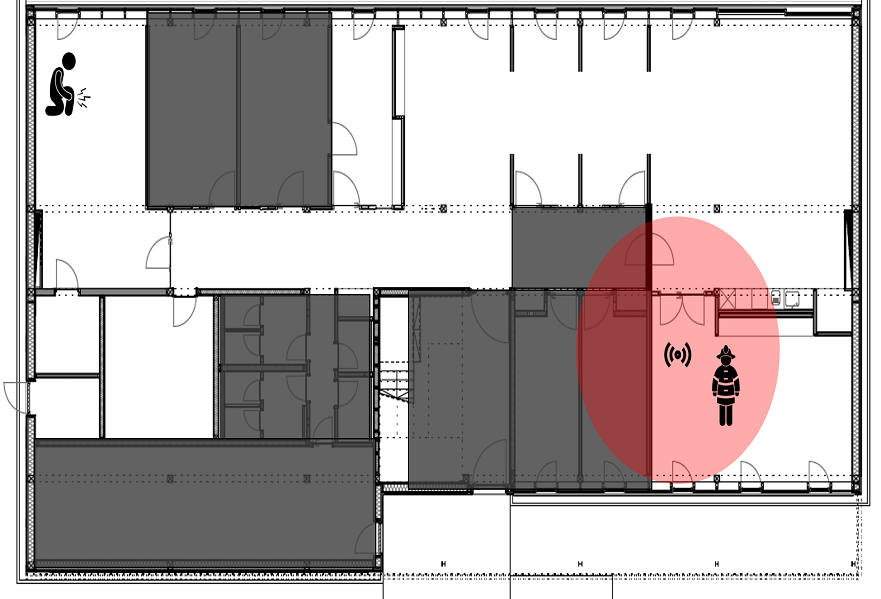
\includegraphics[scale=0.35]{Introduzione/intervento_step_1.png}
		\caption{Rete allo step 1 dell'esploratore}
		\label{fig:step1}
	\end{minipage}
	\ \hspace{10 mm} \
	\begin{minipage}[b]{6cm}
		\centering
		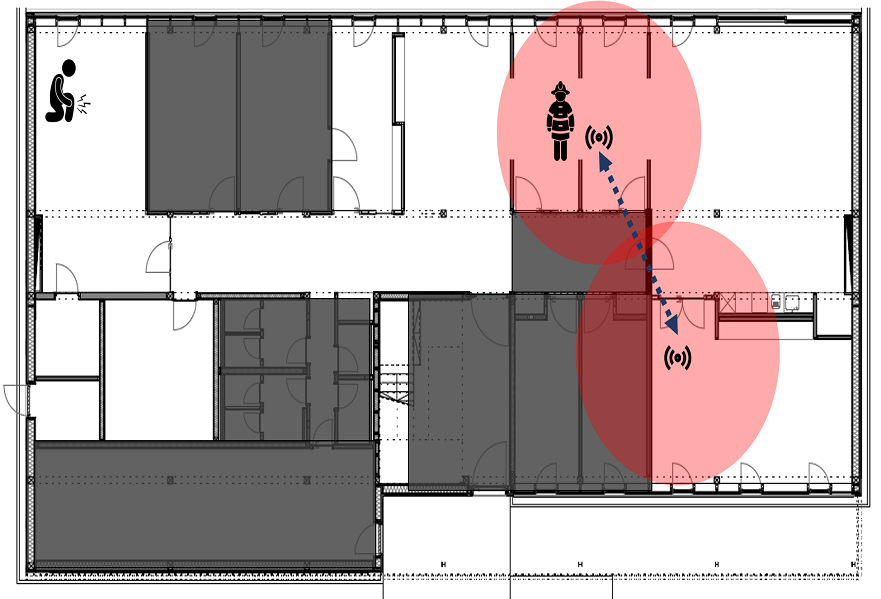
\includegraphics[scale=0.35]{Introduzione/intervento_step_2.png}
		\caption{Rete allo step 1 dell'esploratore}
		\label{fig:step2}
	\end{minipage}
\end{figure}


\begin{figure}[h]
	\begin{minipage}[b]{6cm}
		\centering
		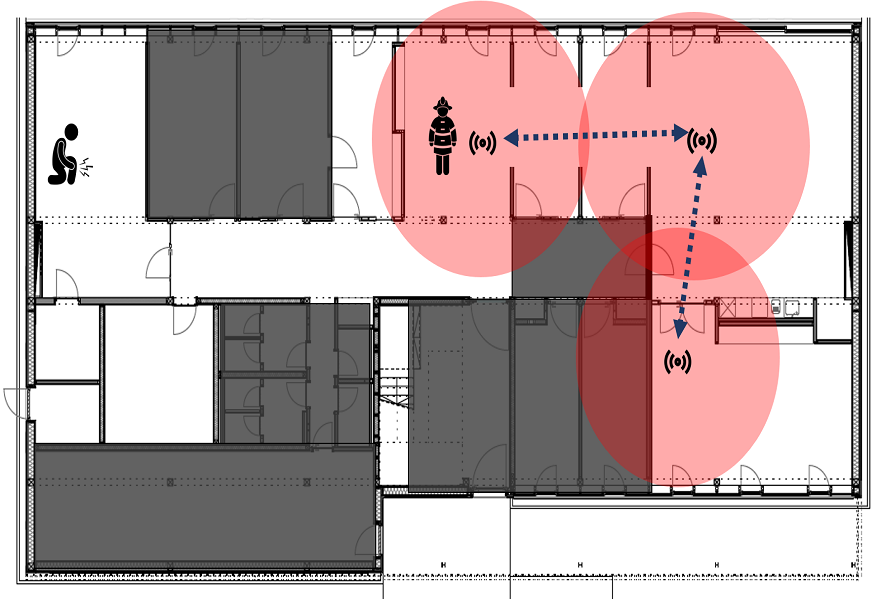
\includegraphics[scale=0.35]{Introduzione/intervento_step_3.png}
		\caption{Rete allo step 3 dell'esploratore}
		\label{fig:step3}
	\end{minipage}
	\ \hspace{10 mm} \
	\begin{minipage}[b]{6cm}
		\centering
		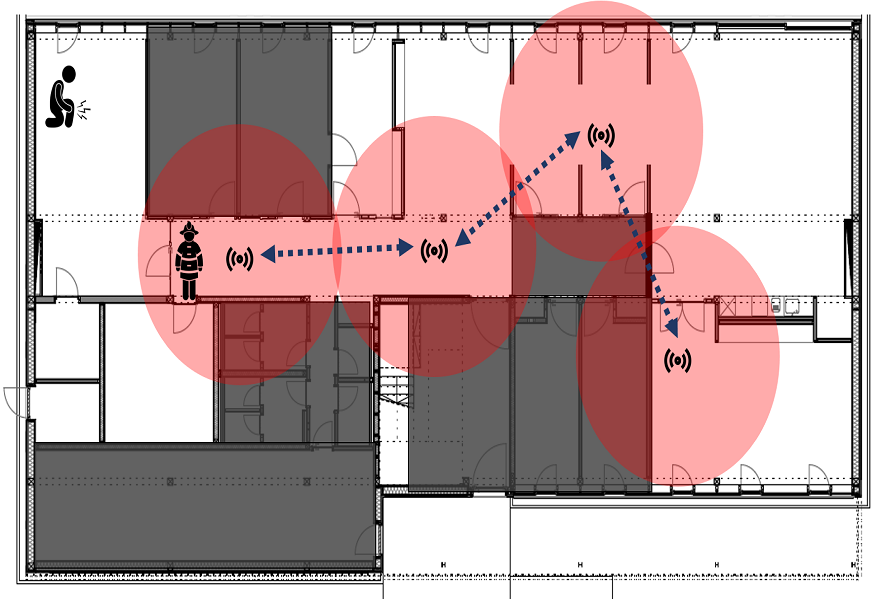
\includegraphics[scale=0.35]{Introduzione/intervento_step_4.png}
		\caption{Rete allo step 4 dell'esploratore}
		\label{fig:step4}
	\end{minipage}
\end{figure}

\begin{figure}[h]
	\begin{minipage}[b]{6cm}
		\centering
		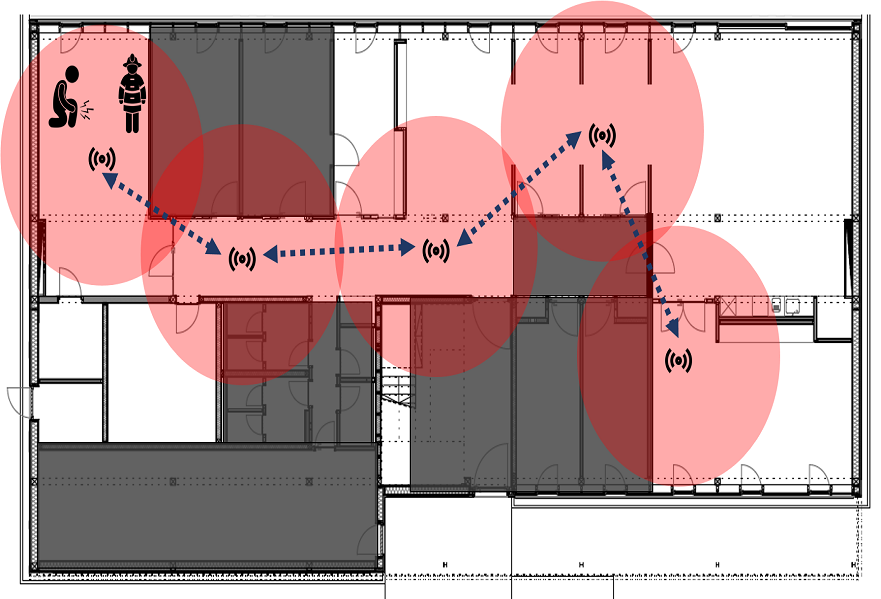
\includegraphics[scale=0.35]{Introduzione/intervento_step_5.png}
		\caption{Rete allo step 5 dell'esploratore}
		\label{fig:step5}
	\end{minipage}
	\ \hspace{10 mm} \
	\begin{minipage}[b]{6cm}
		\centering
		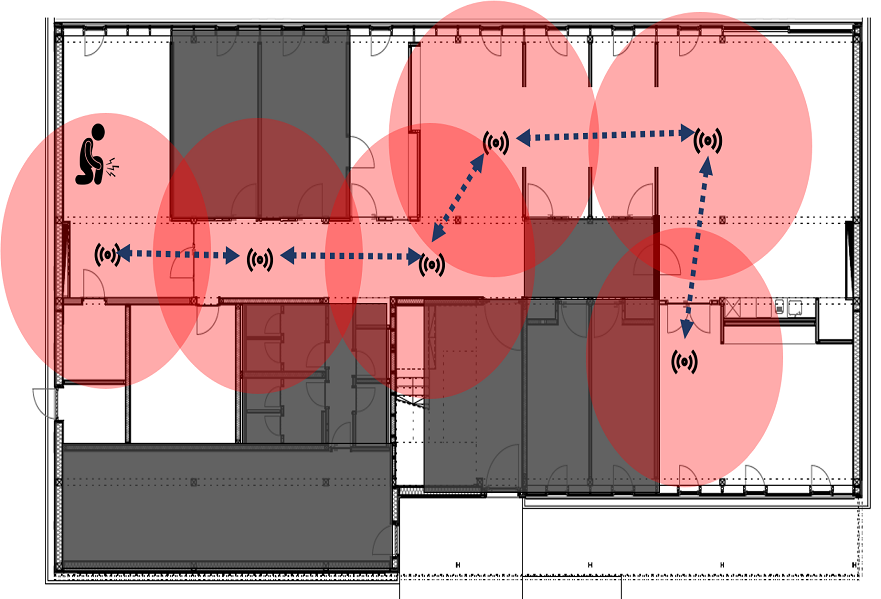
\includegraphics[scale=0.35]{Introduzione/intervento_step_6.png}
		\caption{Rete allo step 6 dell'esploratore}
		\label{fig:step6}
	\end{minipage}
\end{figure}
\newpage
Una volta creata l’infrastruttura, gli operatori potranno comunicare e condividere informazioni come posizione e stato. \newline
La presente tesi è così strutturata:
\begin{description}
\item [Capitolo 1:] Viene descritto il problema della geolocalizzazione indoor, il sistema ideato e le sue parti realizzate nel contesto di questa tesi.
\item [Capitolo 2:] Vengono illustrate le tecnologie utilizzate (sensori MEMS e UWB).
\item [Capitolo 3:] Viene descritto il rumore dei dati grezzi, le tecniche di raffinamento e alcuni algoritmi di data fusion.
\item [Capitolo 4:] Si riporta l'implementazione software e hardware del sottosistema realizzato.
\item [Capitolo 5:] Viene illustrato il procedimento di validazione e l'analisi dei dati ottenuti mediante algoritmi di data fusion.
\end{description}
\chapter{Contesto applicativo }
\label{contesto}
Nella parte iniziale di questo capitolo viene esplicato il contesto applicativo di questa tesi, una volta delineato vengono illustrate le tecniche basilari più utilizzate in questo ambito.

\section{Context-aware computing}
\label{context-aware}
Il sistema realizzato nell'ambito di questa tesi, si colloca nel paradigma di computazione noto come \textit{Context-aware computing}, ovvero un'applicazione nel quale i servizi utilizzano informazioni relative al contesto. In \cite{context} si definisce come \textit{context}:

\begin{quotation}
\textit{Ogni informazione che può essere usata per caratterizzare la situazione di un'entità. Ovvero una persona, un posto o un oggetto che è considerato rilevante all'interazione tra l'utente e l'applicazione, inclusi quest'ultimi.}
\end{quotation}

Questa definizione facilita il lavoro di progettazione e sviluppo di un applicazione permettendo di identificare quali informazioni sono importanti e quali no.
Si consideri un'applicazione nel quale l'utente deve registrare il peso degli oggetti presenti nel magazzino tramite una bilancia come mostrato dalla Fig.\ref{fig:context}:

\begin{figure}[H]  
	\centering 
	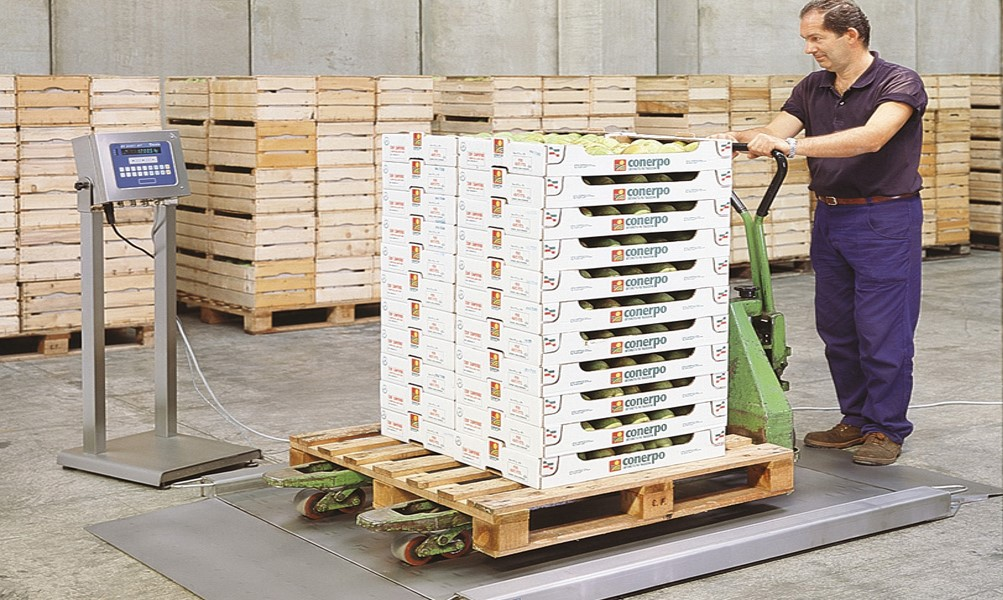
\includegraphics[scale=0.4 ]{ContestoApplicativo/bilancia.jpg}
	\caption{Esempio esplicativo del concetto di contesto}
	\label{fig:context}
\end{figure}
Nello scenario descritto le \textit{entità} sono rispettivamente utente e sistema, mentre due possibili informazioni riguardanti il contesto sono la presenza di altre persone e la posizione geografica del magazzino.\\
La presenza di altre persone nelle vicinanze non influisce il compito dell'utente, quindi non può essere considerato come informazione contestuale. La posizione geografica del magazzino invece si, infatti se quest'ultimo fosse situato in Italia il peso verrebbe calcolato in chilogrammi mentre se fosse situato negli USA verrebbe calcolato in libbre.\\
I sistemi che reperiscono, usano o interpretano queste informazioni contestuali sono detti \textit{context-aware} e vengono definiti in \cite{context} come:
\begin{quotation}
	\textit{Un sistema è context-aware se usa il contesto per fornire informazioni rilevanti e/o servizi agli utenti, dove la rilevanza dipende dal compito degli utenti.}
\end{quotation}
Uno dei tipi di context-aware più utilizzati si basa sul contesto della localizzazione, ovvero servizi basati sulla conoscenza di dove qualcosa o qualcuno si trovi. Nell'era moderna i servizi basati sulla localizzazione (in inglese: Location based services LBSs) stanno assumendo sempre più importanza nelle attività quotidiane dell'uomo grazie alle molteplici possibili applicazioni, tra le quali navigazione assistita per autoveicoli, tracking di persone sensibili (bambini, anziani, malati), servizi di emergenza e così via.\\
I LBSs vengono divisi in due macro categorie:
\begin{itemize}
	\item \textbf{OPSs}: Outdoor Positioning System Service, ovvero servizi di localizzazione in ambienti aperti.
	\item \textbf{IPSs}: Indoor Positioning System Service, ovvero servizi di localizzazione in ambienti indoor.
\end{itemize}
La tecnologia satellitare nota come Global Positioning System (GPS) è la tecnologia dominante negli OPSs. Attraverso una rete dedicata di satelliti artificiali in orbita, fornisce ad un terminale mobile o ricevitore GPS informazioni sulle sue coordinate geografiche ed orario, in ogni condizione meteorologica, ovunque sulla Terra o nelle sue immediate vicinanze ove vi sia un contatto privo di ostacoli con almeno quattro satelliti del sistema. La localizzazione avviene tramite la trasmissione di un segnale radio da parte di ciascun satellite e l'elaborazione dei segnali ricevuti da parte del ricevitore \cite{gps}.\\ 
Il grande limite di questa tecnologia è che i ricevitori devono essere nella line of sight (letteralmente a vista d'occhio) di almeno quattro satelliti nel cielo, questo significa che all'interno di edifici e spazi chiusi il segnale viene attenuato e i sistemi perdono di accuratezza. Quindi la tecnologia GPS non è adatta ai servizi di localizzazione indoor.\\
Il sistema realizzato nell'ambito di questa tesi si colloca nell'ambito degli IPSs approfonditi nel paragrafo successivo.


\section{Indoor Positioning System Service}
\label{IPS}
Un sistema di posizionamento indoor (in inglese: Indoor positioning system o IPS) è un sistema in grado di localizzare \textit{oggetti} o \textit{persone} all'interno di edifici utilizzando onde radio, campi magnetici, segnali acustici e/o altre informazioni raccolte dai sensori all'interno di dispositivi mobili \cite{IPS} o da altri  appositamente installati nell'ambiente. Questi sono una specializzazione dei più generici sistemi \textbf{RTLS}, standardizzati dall'\textit{International
Organization for Standardization and the International Electro Technical Commission} (ISO/IEC 24730). Lo standard definisce i sistemi RTLS come:
\begin{quotation}
	\textit{“ I Real time locating system sono sistemi wireless con l'abilità di localizzare la posizione di oggetti ovunque essi siano in uno spazio definito in un certo momento che è, o si avvicina, real time. La posizione è derivata dalla misurazione delle proprietà fisiche del collegamento radio."}
\end{quotation}
La differenza tra RTLS e IPS è che i primi sono stati pensati per le compagnie che vogliono tracciare i propri oggetti e le persone, fornendo uno storico di dove sono stati e dove si trovano ora, mentre gli IPS sono pensati per essere utilizzati da utenti su dispositivi mobili per navigare ed orientarsi all'interno di edifici.
Come già accennato, gli IPS \cite{IPS2} permettono di creare una vasta gamma di servizi, ad esempio:
\begin{itemize}
	\item\textbf{Way-Finding}: permettere di navigare in edifici complessi, come ad esempio aeroporti, seguendo il percorso indicato.
	\item\textbf{Ricerca dei punti d'interesse}, aumentare la customer experience facendo trovare all’utente ciò che desidera.
	\item \textbf{Multi-Dot}: visualizzare in una mappa le posizioni degli utenti per tracciare persone potenzialmente in pericolo (bambini, anziani).
	\item \textbf{Marketing di prossimità}: realizzare marketing mirati, inviando annunci sulle ultime offerte.
\end{itemize}
L’elenco di cui sopra rappresenta solo un ridotto sottoinsieme dei potenziali campi applicativi (vedi Fig.\ref{fig:surveyApplication}), per questo motivo negli ultimi anni \cite{indoorThesis} l'interesse nella ricerca e nello sviluppo di sistemi di questo tipo è cresciuto sempre più tra le aziende, che hanno percepito la possibilità di grandi profitti in un mercato non ancora esplorato del tutto.
\begin{figure}[H]  
	\centering 
	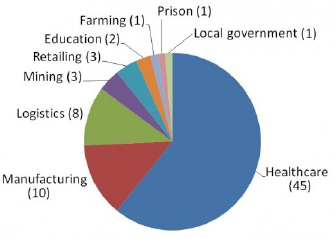
\includegraphics[scale=1.2]{ContestoApplicativo/application.png}
	\caption{Sondaggio tra 74 casi di studio di applicazioni IPS \cite{market}}
	\label{fig:surveyApplication}
\end{figure}

Secondo un sondaggio  di \textit{Markets and Markets} e un articolo pubblicato da\textit{ The International News Magazine}, il mercato degli IPS subirà una crescita annuale media del 42.1\% arrivando a valere 2.60 bilioni di dollari nel 2018. Questo da un'idea del perché grandi aziende come Google, Sony, Microsoft e Apple stiano investendo in questo settore.\\
Un'ulteriore spinta è data dal fatto che, al contrario del GPS per gli OPS (vedi \ref{context-aware}), tuttora non esiste uno standard di riferimento per gli IPS. Infatti sul mercato sono disponibili diversi tipi di IPS commerciali che si differenziano in base al principio di funzionamento e alle tecniche utilizzate, utilizzando hardware specifico o la combinazione di più sistemi.\\ 




\section{Stima della posizione}
\label{metodi_distanza}
Gli IPS possono essere classificati sulla base di diversi fattori, uno di questi è su come determinano la posizione dei.\\
Stimare \cite{IPS2} la distanza tra dispositivi wireless è utile perché attraverso questa informazione è possibile determinarne (con un certo errore) la posizione di un ricevitore rispetto ad un trasmettitore (\cite{alg1}, \cite{alg2}), queste tecniche si distinguono in:

	\begin{itemize}
	\item \textbf{Range based}:
	
		\begin{itemize}
		\item \textit{RSSI}- potenza del segnale radio ricevuto(sez.\ref{rssi})
		\item \textit{ToA} - tempo d’arrivo: (sez.\ref{toa})
		\item \textit{TDoA} - differenze del tempo di arrivo (sez.\ref{tdoa});
 	    \end{itemize}
     
	\item \textbf{Angle based}:
		\begin{itemize}
			\item \textit{AoA} - Angle of Arrival (sez.\ref{aoa}).
		\end{itemize}
		
\end{itemize}
Per poter determinare le distanze si devono distinguere i punti di riferimento (che hanno
delle coordinate note) dai nodi senza posizione nota a cui assegnare delle coordinate.
Si dicono:
\begin{itemize}
	\item \textbf{Anchor}: i nodi le cui coordinate sono note
	\item \textbf{Target}: il nodo di cui non si conosce la posizione.
\end{itemize}

 L’obiettivo del posizionamento è assegnare le giuste coordinate agli Unknown rispetto ad un sistema di riferimento. Questo è strettamente legato all'implementazione dell'IPS e così anche la codifica delle posizioni all'interno del sistema di riferimento, le coordinate potrebbero essere restituite all'utente in maniera relativa ("vicino alla cucina") oppure assoluta ("tre  metri in direzione ovest dal nodo 1").

\subsection{Range based}
Nel posizionamento dei nodi basato sulla distanza la stima della posizione del target dipende dai seguenti parametri:
	\begin{itemize}
	\item il tempo trascorso tra l’emissione e la ricezione del segnale radio;
	\item la distanza euclidea tra ogni emettitore ed il ricevitore;
	\item la potenza del segnale ricevuto.
\end{itemize}
In alcuni casi sono necessarie tre o più Anchor per ottenere le coordinate da assegnare allo Unknown.

\subsubsection{Received Signal Strength Indicator - RSSI}
\label{rssi}
La comunicazione \cite{IPS2} tra dispositivi wireless (senza fili) avviene tramite lo scambio di segnali propagati nell’aria. Durante la propagazione i segnali tendono ad attenuarsi con l'aumentare della distanza percorsa fino a non essere più percepibili.

\begin{figure}[H]  
	\centering 
	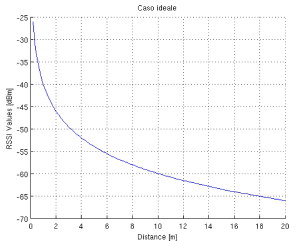
\includegraphics[scale=1.2]{ContestoApplicativo/signal.PNG}
	\caption{RSSI - Andamento della potenza in funzione della distanza percorsa dal segnale}
	\label{fig:signal}
\end{figure}

La stima della potenza del segnale ricevuto è data dall’indicatore RSSI \cite{rssi}. La distanza emettitore-ricevitore si stima utilizzando \textbf{l’equazione di trasmissione di Friis}.

\begin{equation}
		P_{T}=P_{R} \dfrac{G_{T}G_{R}\lambda^2}{(4\pi)^2d^n}
		\label{eq1}
\end{equation}

dove:
\begin{itemize}
	\item $P_{R}$: potenza del segnale ricevuto (Watt)
	\item $P_{T}$: potenza del segnale trasmesso(Watt)
	\item $G_{R}$: guadagno dell'antenna ricevente
	\item $G_{T}$: guadagno dell'antenna trasmittente
	\item $\lambda=\frac{v}{f}$: lunghezza d'onda, dove $v$ è la velocità di propagazione e $f$ è la frequenza dell'onda
	\item $d$: distanza espressa in metri
	\item $n$: constante di propagazione del segnale che dipende dall'ambiente 
\end{itemize}

Con la seguente equazione invece è possibile convertire la potenza espressa in Watt nella potenza espressa in dBm:
\begin{equation}
P[dBm] = 10\log_{10}(10^3P[W])
\label{eq2}
\end{equation}
Combinando l'equazione \ref{eq1} con \ref{eq2} e applicando le proprietà dei logaritmi si ottiene:
\begin{equation}
RSSI = -(10 n \log_{10} d - A)
\label{eq3}
\end{equation}
dove $A$ è la potenza del segnale ricevuto a distanza fissa di un metro (espressa in dBm), considerando una costante di propagazione $n$.\\
La stima della distanza si ottiene infine dalla seguente equazione:
\begin{equation}
d = 10 (\frac{A - RSSI}{10n})
\label{eq4}
\end{equation}
Tuttavia la distanza restituita non è del tutto precisa, infatti la potenza del segnale potrebbe essere alterata dall'ambiente circostante attraverso i fenomeni di \textbf{Riflessione} (il segnale sbatte e si riflette su vari ostacoli seguendo più percorsi) e di \textbf{Assorbimento} (il decadimento viene alterato dagli oggetti presenti). Tale tecnica viene solitamente completata utilizzando il metodo della \textbf{Trilaterazione} (sez.\ref{trilaterazione})\\


\subsubsection{Time Of Arrival measurements}  
\label{toa}
A differenza del precedente metodo, con questa tecnica la distanza tra emettitore e ricevitore viene stimata sulla base del tempo impiegato dal segnale a raggiungere il ricevitore. Nello specifico la sequenza di azioni è:
\begin{enumerate}
	\item Il nodo \textit{A} invia il segnale al tempo $t_1$
	\item Il segnale arriva al nodo \textit{B} al tempo $t_2$
	\item \textit{B} elabora il messaggio impiegando un tempo $t_d$ e lo invia al tempo $t_3$
	\item Il segnale torna al nodo \textit{A} al tempo $t_4$
\end{enumerate}
Come mostrato dalla figura seguente:

\begin{figure}[H]  
	\centering 
	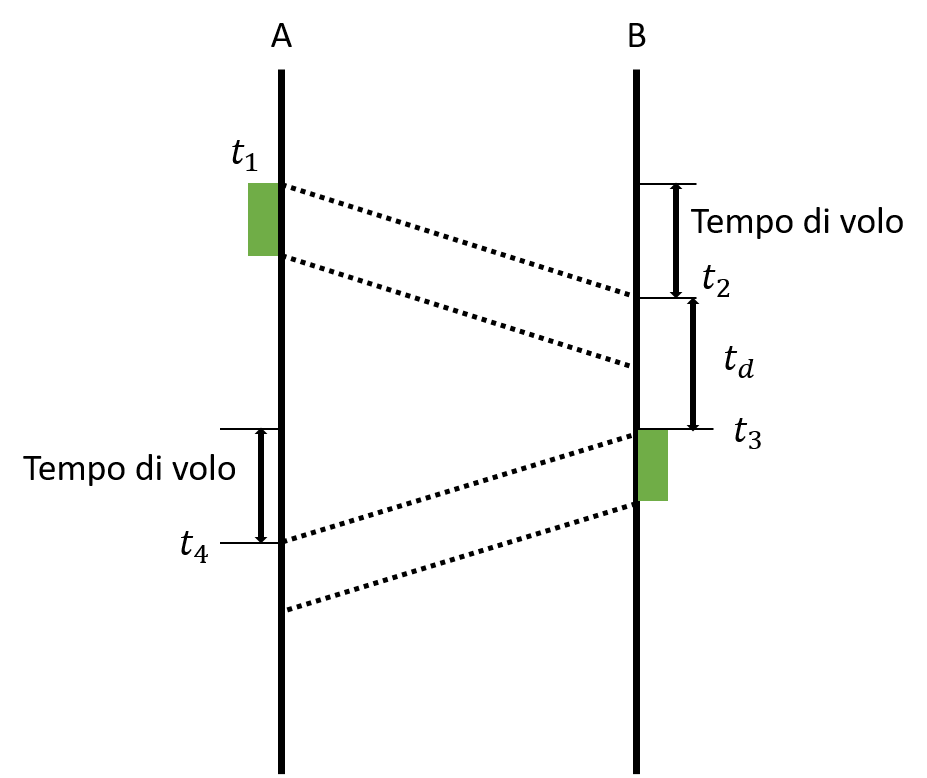
\includegraphics[scale=0.4]{ContestoApplicativo/toa.png}
	\caption{ToA - Principio di funzionamento}
	\label{fig:toa}
\end{figure}

Quindi il tempo di viaggio può essere ricavato con la seguente equazione:

\begin{equation}
t_d = \dfrac{(t_4 - t_1) - (t_3 - t_2)}{2}
\label{td}
\end{equation}

E infine la distanza stimata attraverso:
\begin{equation}
d_{ToA} = t_d * c
\label{eq:toa}
\end{equation}

dove $c$ è la velocità di propagazione della luce nel vuoto pari a 299792458 m/s. Per identificare in modo univoco un target, questa tecnica viene completata dalla tecnica di posizionamento nota come \textbf{Trilaterazione} (sez. \ref{trilaterazione}), come per le misure RSSI viste precedentemente.\\
Il difetto principale di questa tecnica consiste nel fatto che sistemi utilizzati devono avere un complesso meccanismo di sincronizzazione per mantenere una fonte affidabile di tempo per i sensori\cite{toaProblem}.

\subsubsection{Time Difference Of Arrival}
\label{tdoa}
Questa tecnica è basata sulla differenza nel tempo di arrivo di un segnale emesso da due sorgenti diverse verso un altro nodo, come mostrato in Fig.\ref{fig:tdoa}).

\begin{figure}[H]  
	\centering 
	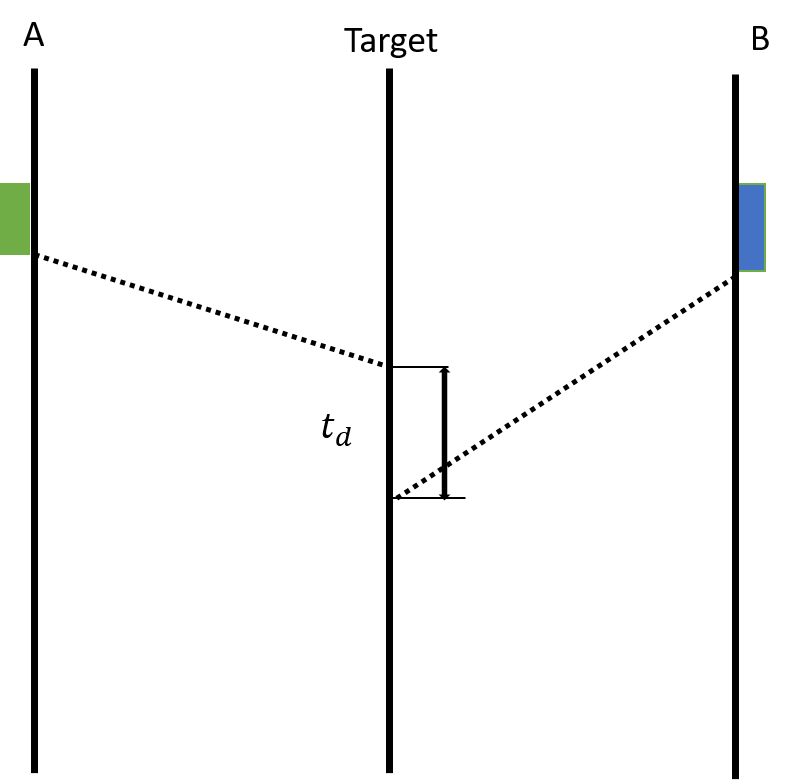
\includegraphics[scale=0.4]{ContestoApplicativo/tdoa.png}
	\caption{TDoA - Principio di funzionamento}
	\label{fig:tdoa}
\end{figure}
Se si suppongono note le posizioni dei nodi \textit{A} e \textit{B} rispetto ad un sistema di riferimento, indicate rispettivamente dalle tuple $(x_B,y_B)$ e $(x_A,y_A)$, la distanza del nodo \textit{Target} può essere stimata dalla seguente equazione:
 
\begin{equation}
\Delta d = \Delta t_d * c
\label{eq:tdoa}
\end{equation}

Dove:
\begin{itemize}
	\item $c$ è la velocità di propagazione della luce nel vuoto
	\item $ \Delta t$ è la differenza del tempo di arrivo dei segnali emessi dai nodi \textit{A} e \textit{B}
	\item $\Delta d$ è la distanza in due dimensioni: $(\sqrt{(x_B-x)^2 + (y_B-y)^2}- \sqrt{(x_A-x)^2 + (y_A-y)^2})$ 
\end{itemize}

In questo modo, la posizione del \textit{target} viene stimata all'interno del luogo geometrico dei punti del piano aventi come costante la differenza delle distanze tra i nodi, ovvero dall'iperbole avente come fuochi i nodi \textit{A} e \textit{B}. Come mostrato in Fig.

\begin{figure}[H]  
	\centering 
	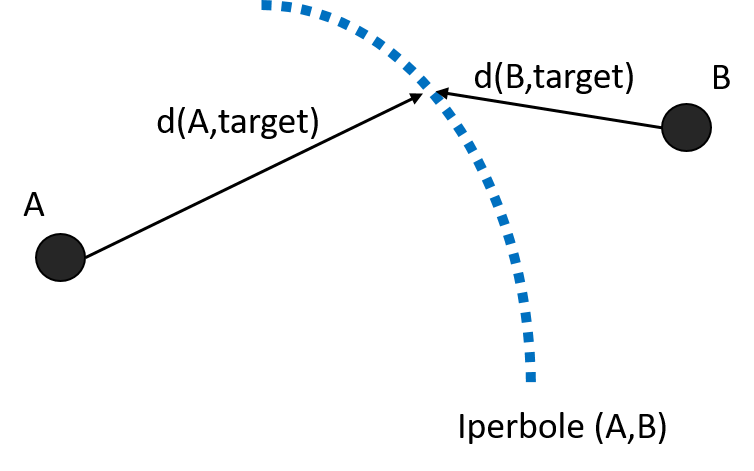
\includegraphics[scale=0.4]{ContestoApplicativo/tdoa1.png}
	\caption{TDoA - Stima della posizione lungo l'iperbole identificata da due nodi}
	\label{fig:tdoa1}
\end{figure}

	Tuttavia così facendo la posizione del \textit{target} rimane stimata in un'insieme di punti infinito, quindi come per le tecniche viste precedentemente (\ref{rssi} e \ref{toa}) per identificare in modo univoco il target questa tecnica ha bisogno di essere completata dalla tecnica di posizionamento nota come \textbf{Trilaterazione} \ref{trilaterazione}.

\subsection{Angle Based}
\label{angle}
\subsubsection{Angle of Arrival}
\label{aoa}
Con questa tecnica la posizione del \textit{target} viene stimata misurando gli angoli di incidenza del segnale trasmesso ad altri nodi.\\
Si consideri \cite{aoa} un antenna in un canale di propagazione, la tensione del segnale ricevuto (\ref{fig:aoa}) è data dalla seguente equazione:\\
\begin{equation}
 V = \int_{0}^{2\pi} AoA(\varphi) G(\varphi)d\varphi 
\end{equation}

Dove:
\begin{itemize}
	\item $AoA(\varphi)$ rappresenta l'ampiezza e la fase dell'onda incidente
	\item $G(\varphi)$ è il campo elettrico del nodo target 
	\item $C$ valore proporzionale constante
\end{itemize}

Se si ruota l'antenna di un angolo $\alpha$ intorno a se stessa nel piano cartesiano la precedente equazione diventa:
\begin{equation}
\label{eq:2}
V (\alpha) = \int_{0}^{2\pi} AoA(\alpha-\varphi) G(\varphi)d\varphi 
\end{equation}

Possiamo notare che l'Eq.\ref{eq:2} è la convoluzione di $AoA$ e $G$ e può essere scritta nel seguente modo:
\begin{equation}
\label{eq:3}
V (\alpha) = C AoA(\alpha) * G(\alpha)
\end{equation}

Si è scelto di normalizzare l'Eq.\ref{eq:3} con il valore constante $C$. Quindi, utilizzando la transformata di Fourier l'Eq.\ref{eq:3} diventa:

\begin{equation}
\label{eq:4}
F(V(\alpha)) = F(AoA(\alpha)) F(G(\alpha))
\end{equation}

Da cui è possibile calcolare l'angolo di incidenza desiderato:

\begin{equation}
\label{eq:5}
AoA(\alpha) = F^{-1} \dfrac{F(V(\alpha))}{F(G(\alpha))} \quad se \quad F(G(\alpha))\neq 0
\end{equation}

\begin{figure}[H]  
	\centering 
	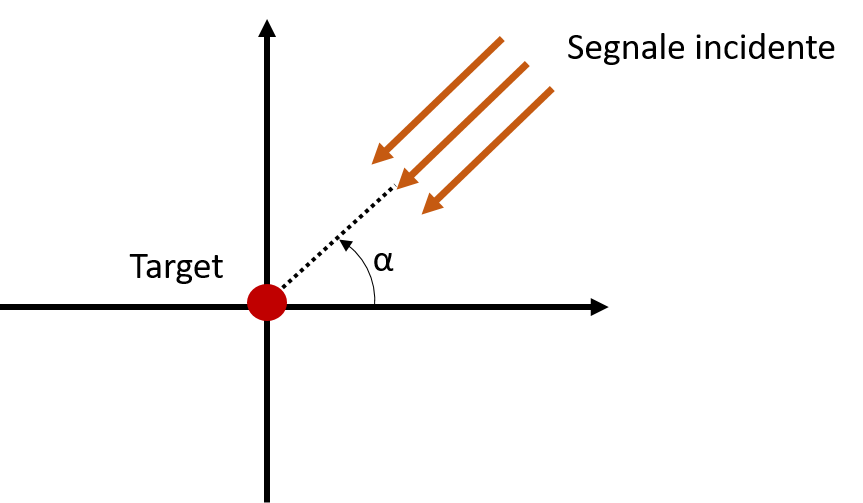
\includegraphics[scale=0.4]{ContestoApplicativo/aoa.png}
	\caption{AoA - Stima della posizione attraverso l'angolo di incidenza}
	\label{fig:aoa}
\end{figure}

Il vantaggio dell’AoA risiede nella possibilità di ottenere un risultato attendibile senza la necessità di informazioni riguardanti i tempi di trasmissione. A fronte del risparmio dal punto di vista computazionale, la tecnica presenta alcuni svantaggi pratici, dovuti al costo dell’hardware, che al fine di restituire informazioni precise, deve essere di alta qualità; rischiando altrimenti di incorrere in fenomeni che comprometterebbero la misurazione. Per questo motivo solitamente questa tecnica viene completata dalla tecnica di posizionamento nota come \textit{Triangolazione} (\ref{triangolazione}).


\section{Tecniche di localizzazione}
Per tecniche di localizzazione si intendono tutte quelle tecniche che, combinate alle differenti metodologie di stima della posizione viste precedentemente (vedi \ref{metodi_distanza}), permettono di localizzare un nodo \textit{target} all'interno di un sistema di riferimento.\\
In questo paragrafo vengono illustrate quelle più conosciute e basilari nell'ambito degli IPS.

\subsection{MIN-MAX}
Combina le stime della distanza di più \textit{anchor}, ottenute attraverso tecnica \textit{RSSI} (\ref{rssi}), nel seguente modo:

\begin{itemize}
	\item Stimare la distanza $d_i$ di ogni nodo i-esimo in base al valore RSSI
	\item Traccia due linee orizzontali e verticali a distanza $d_i$ dallo nodo \textit{target}
	\item Identifica un quadrato di lato 2  $d_i$ i cui estremi saranno: \\
			$[max(x_i-d:i),max(y_i-d_i)] * [min(x_i+d_i),min(y_i+d_i))]$
	\item Calcola le intersezioni dei quadrati
\end{itemize}

Il centro del quadrato (Fig.\ref{fig:minmax}) rappresenta la posizione stimata del \textit{target}. Più piccola sarà l’area e maggiore sarà l’accuratezza della posizione stimata.
\begin{figure}[H]  
	\centering 
	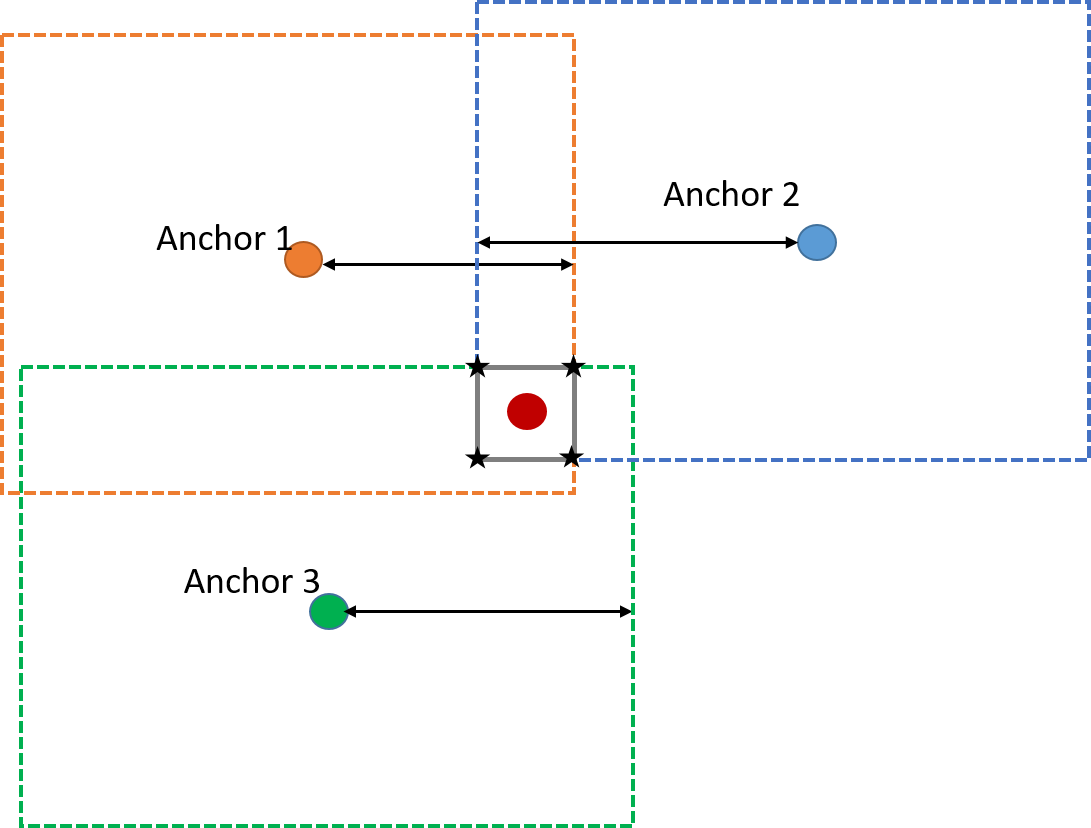
\includegraphics[scale=0.4]{ContestoApplicativo/minmax.png}
	\caption{MIN-MAX - Tecnica di posizionamento }
	\label{fig:minmax}
\end{figure}



\subsection{Trilaterazione}
\label{trilaterazione}
Consideriamo 3 \textit{Anchor} intorno cui disegniamo 3 circonferenze aventi per centro le coordinate degli \textit{Anchor} e per raggio l'RSSI del segnale ricevuto dallo \textit{Uknown}, come mostrato in figura:
\begin{figure}[H]  
	\centering 
	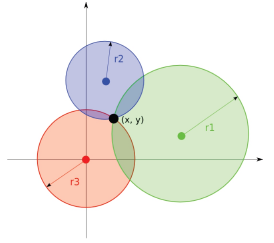
\includegraphics[scale=0.8]{ContestoApplicativo/trilaterazione.png}
	\caption{Trilaterazione - Esempio esplicativo}
	\label{fig:trilaterazione}
\end{figure}
Quindi le coordinate dell'Unknown sono la soluzione del seguente sistema:
\begin{equation}
\begin{cases}
(x-x_1)^2 + (y-y_1)^2 = r_1^2\\
(x-x_2)^2 + (y-y_2)^2 = r_2^2\\
(x-x_3)^2 + (y-y_3)^2 = r_3^2
\end{cases}
\end{equation}
In base alla soluzione del sistema si può avere una delle seguenti situazioni:
\begin{itemize}
	\item La soluzione non è unica, si hanno tre cerchi che si sovrappongono
	\item Il sistema non ammette soluzione, i raggi vanno aumentati
	\item La soluzione esiste ed è unica, i tre cerchi si intersecano in un solo punto
\end{itemize}



\subsection{Triangolazione}
\label{triangolazione}
A differenza delle Trilaterazione (\ref{trilaterazione}), queste tecniche identificano la posizione del nodo \textit{target} a partire dagli angoli stimati da tre anchors attraverso una delle teniche Angle Based (\ref{angle}).\\
In \cite{triangolazione} si descrive la triangolazione geometrica attraverso il seguente algoritmo:\\

\begin{enumerate}
   \item Siano \textit{1,2 e 3} le anchor in grado di stimare l'angolo, rispetto ad una circonferenza concentrica all'anchor stessa, del nodo target
   \item siano $L_{12}$ e $L_{31}$ rispettivamente le distanze tra l'anchor 1 e 2 e l'anchor 3 e 1
   \item Siano gli angoli compresi tra \textit{1} e \textit{2} e tra \textit{1} e \textit{3}, indicati rispettivamente con $\lambda_{12} e \lambda_{13}$, minori di 180°
   \item sia $\phi$ l'angolo tra l'asse x positivo e la linea formata dall'anchor \textit{1} e \textit{2}
   \item sia $\sigma$ l'angoolo tra l'asse x positivo, l'anchor \textit{1} e l'anchor \textit{3} più $\phi$
   \item sia $\gamma= \sigma - \lambda_{31}$
   \item sia $p= \dfrac{L_{31} \sin\lambda_{12}}{L_{12} \sin\lambda_{31}}$
   \item sia $\tau= \tan^{-1} \dfrac{\sin\lambda{12}-p \sin\gamma}{p \cos\gamma-\cos\lambda{12}}$
   \item sia $L_1 = \dfrac{L_{12} sin(\tau+\lambda_{12})}{\sin\lambda_{12}}$
\end{enumerate}

Allora le coordinate $x$ e $y$ del target sono date da:
\begin{itemize}
	\item $x_R = x_1 - L_1  \cos(\phi + \tau)$
	\item $y_R = y_1 - L_1  \sin(\phi + \tau)$
	\item $\Phi_R = \phi + \tau - \lambda_1$
\end{itemize}
Dove $\Phi_R$ rappresenta l'orientamento del nodo target, come mostrato in Fig.\ref{fig:triangolazione}.


\begin{figure}[H]  
	\centering 
	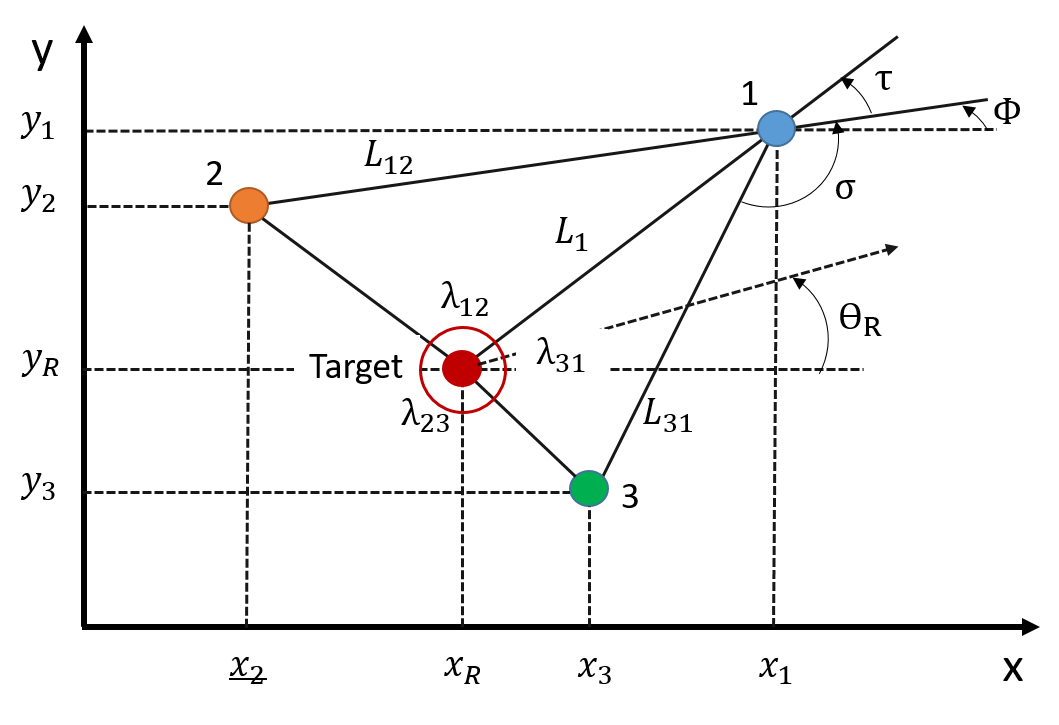
\includegraphics[scale=0.4]{ContestoApplicativo/triangolazione.png}
	\caption{Triangolazione - Esempio esplicativo}
	\label{fig:triangolazione}
\end{figure}





\section{Sensor Data Fusion}

In generale con Sensor Data Fusion si indicano tutte quelle tecniche che \cite{sensorfusion} combinano dati provenienti da sensori o derivate da altre risorse tali che l'informazione risultante ha una minore incertezza rispetto a quella ottenuta utilizzando le risorse individualmente. \\
Nel contesto degli IPS (\ref{IPS}), il Sensor Fusion ha come scopo quello di determinare informazioni riguardanti la posizione di oggetti e/o persone. Le risorse delle informazioni grezze sono le più svariate, tra le quali:
\begin{itemize}
	\item Accelerometro
	\item Giroscopio
	\item Magnetometro
	\item Infrarossi
	\item RFID 
	\item Sensori ottici
	\item Sensori di pressione
	\item Bluetooth
	\item WiFi
	\item Telecamera
	\item UWB
\end{itemize}

Come e quali risorse utilizzare per stimare la posizione di un oggetto è una sfida ingegneristica non banale, ma grazie alla crescente richiesta di IPSs la ricerca di nuove tecnologie e algoritmi in questo settore ha permesso di raggiungere risultati incredibili fino a qualche anno. \\








\chapter{Descrizione del sistema}
\label{scenario}
In questo capitolo si illustra inizialmente il macrosistema inerente al progetto aziendale, con tutti i suoi sottosistemi e i loro rispettivi obiettivi. Nel paragrafo successivo invece, viene approfondito il sottosistema realizzato specificandone i requisiti funzionali e non. 


\section{Il macrosistema}



\section{Il sistema realizzato}
\chapter{Unità di misura inerziale}
\label{tecnologie}
Le unità di misura inerziale \cite{mems} (in inglese Inertial Measurement Units - IMU) sono dispositivi elettronici basati su sensori inerziali come accelerometri (\ref{accell}) e giroscopi (\ref{giroscopi}). In molti casi a questi vengono aggiunti altri sensori utili ad applicazioni di navigazione come il magnetometro (\ref{magnetometro}). Nello specifico di questa tesi, l'IMU utilizzata è un circuito integrato composto da questi tre sensori (più altri non utilizzati come sensore di temperatura) realizzati tramite tecnologia MEMS (acronimo di Microelectro Mechanical System, ovvero sistemi meccanici microelettrici).\\
Nel corso degli anni l'interesse per questa tecnologia è cresciuto grazie ai vantaggi in termini economici e tecnici, tra questi i più importanti sono:
\begin{itemize}
	\item costo di realizzazione costante e proporzionale alla superficie del dispositivo
	\item grande potenziale di integrazione nei circuiti elettronici integrati
	\item basso consumo energetico
	\item dimensioni ridotte
\end{itemize}
 
 In questo capitolo si illustrano i principi di funzionamento alla base dei sensori, realizzati mediante tecnologia MEMS, integrati nell'IMU utilizzata nel lavoro di questa tesi.



\section{Accelerometro}
\label{accell}
In generale un accelerometro è un dispositivo in grado di misurare l’accelerazione di un corpo rigido causata da una forza esterna. Questa può essere statica, come la forza di gravità, o dinamica nel caso di forze vibranti applicate al dispositivo.\\
Uno dei più comuni accelerometri MEMS è quello \textit{capacitivo} che, come il nome suggerisce, si basa sulla \textit{capacità} elettrostatica. Se due piastre sono posizionate parallelamente tra di loro e poste ad una certa distanza, allora la capacità generata è data da:

\begin{equation}
\label{capacita}
C = \varepsilon_r \varepsilon_0 \dfrac{A}{d} 
\end{equation}
Dove:
\begin{itemize}
	\item $C$ è la capacità
	\item $\varepsilon_0$ è la constante dielettrica del vuoto
	\item $\varepsilon_r$ è la constante dielettrica relativa al materiale utilizzato per le piastre
	\item $A$ è l'area delle piastre
	\item $d$ è la distanza tra le due piastre
\end{itemize}
Dall'Eq.\ref{capacita} si noti che la capacità può variare solo se vi sono cambiamenti nell'area delle piastre o nella loro distanza. Proprio su quest'ultimo parametro si basano gli accelerometri capacitivi. Una classica struttura è rappresentata dalla Fig.\ref{fig:acc1}:
 \begin{figure}[H]  
	\centering 
	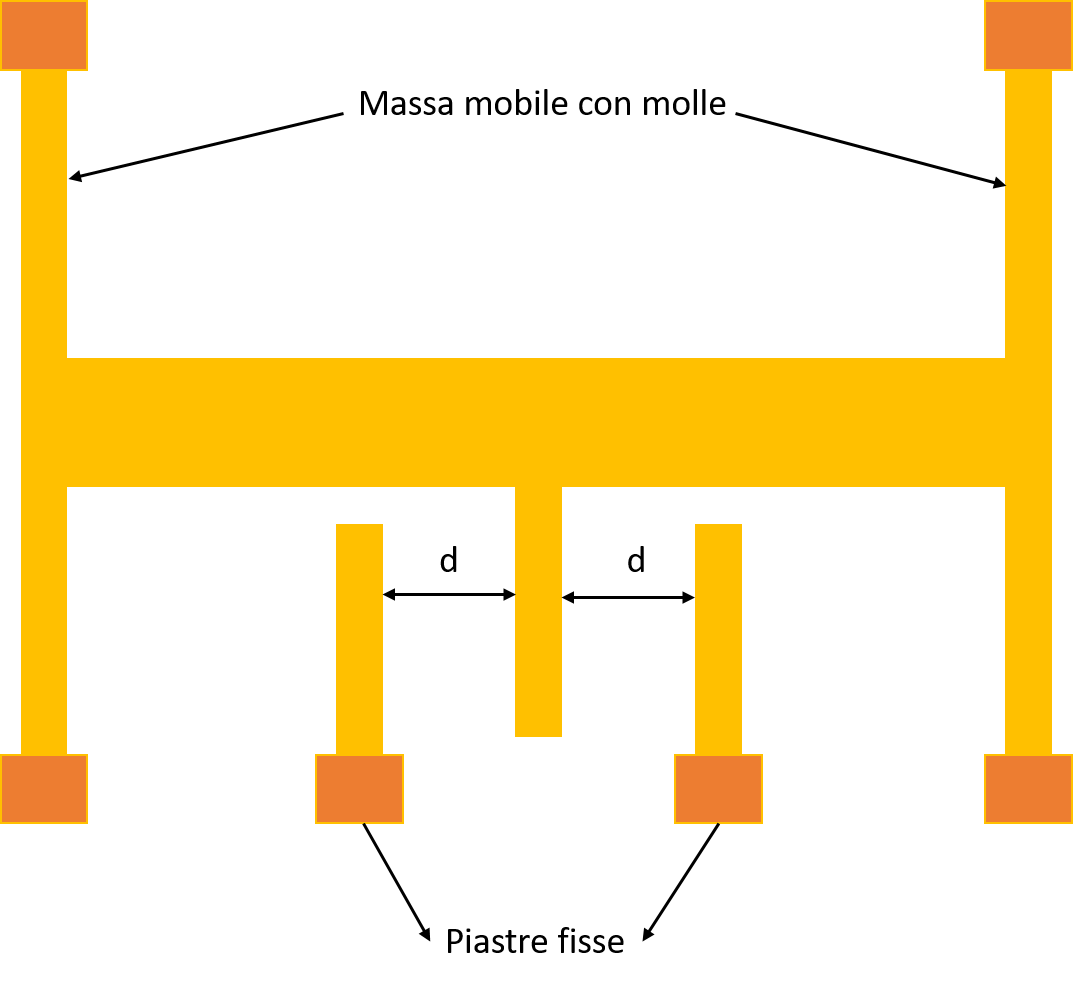
\includegraphics[scale=0.25 ]{tecnologie/acc1.png}
	\caption{Rappresentazione esemplificativa di un accelerometro capacitivo a riposo}
	\label{fig:acc1}
\end{figure}
La massa centrale è in grado di muoversi lungo un asse orizzontale grazie a delle molle poste alle sue estremità, come rappresentato in Fig.\ref{fig:acc2}:
 \begin{figure}[H]  
	\centering 
	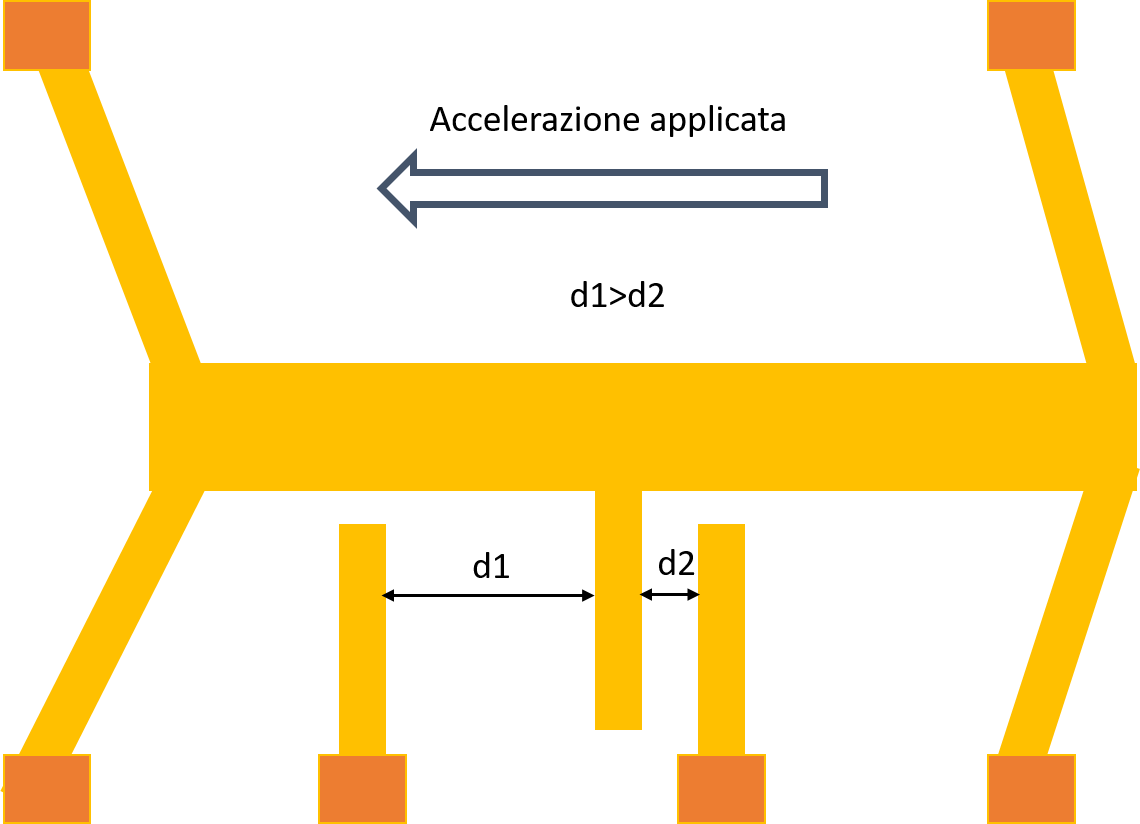
\includegraphics[scale=0.25 ]{tecnologie/acc2.png}
	\caption{Rappresentazione esemplificativa di un accelerometro capacitivo che subisce una forza esterna}
	\label{fig:acc2}
\end{figure}

A seguito del movimento della massa centrale, la distanza $d2$ in Fig.\ref{fig:acc2} si farà più piccola provocando una variazione di tensione ai capi della massa centrale. Questa verrà quindi convertita in un valore numerico rappresentante l'accelerazione subita in base alla scala e alla sensibilità del dispositivo.\\ 

\section{Giroscopio}
\label{giroscopi}
In generale, un giroscopio è un dispositivo in grado di misurare la velocità angolare a cui è sottoposto il dispositivo. I giroscopi realizzati mediante tecnologia MEMS si basano sulla forza di \textit{Coriolis}. In fisica \cite{corolois}, la forza di Coriolis è una forza apparente a cui risulta soggetto un corpo quando si osserva il suo moto da un sistema di riferimento che sia in moto circolare rispetto ad un sistema di riferimento inerziale. \\
I giroscopi di questo tipo sono composti \cite{gyroMems} da una \textit{massa} \textbf{m}, due \textit{molle} e due ammortizzatori come mostrato in Fig.\ref{fig:gyro}. Si assuma  l'asse x come l'asse di direzione (drive mode) e l'asse y come l'asse di rilevamento(sensing mode). Quando la massa è sottoposta ad una vibrazione armonica applicata da una forza elettrostatica, elettromagnetica o elettrotermica, lo spostamento lungo l'asse x è dato da:
\begin{equation}
x(t) = A_x \cos(\omega_x t)
\end{equation}
Dove $A_x$ è l'ampiezza e $\omega_x$ è la frequenza angolare.  Una velocità angolare $\Omega_z$ in input intorno all'asse z causa un'accelerazione di Coriolis lungo l'asse y data dalla seguente equazione:
\begin{equation}
a_y= 2\Omega_z \times \frac{d_x}{d_t}= -2\Omega_z A_x \omega_x \sin(\omega_x t)
\end{equation}

La massa quindi inizierà a vibrare lungo l'asse y a causa della forza di Coriolis e la velocità angolare $\Omega_z$ può essere calcolata misurando lo spostamento lungo l'asse vibrante. \\
Quando il \textit{drive mode} e il \textit{sense mode} sono perfettamente uguali ($\omega_x = \omega_y$), l'ampiezza lungo l'asse y raggiunge il massimo mentre la larghezza di banda raggiunge il minimo. In generale, questi due parametri dovrebbero essere uguali al fine di ottimizzare la sensibilità e la larghezza di banda.
 \begin{figure}[H]  
	\centering 
	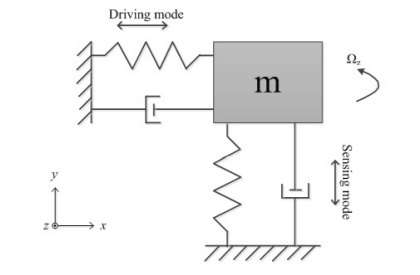
\includegraphics[scale=1]{tecnologie/gyro.png}
	\caption{Rappresentazione di un giroscopio vibrante per la misura della velocità angolare lungo l'asse z}
	\label{fig:gyro}
\end{figure}




\section{Magnetometro}
\label{magnetometro}
In generale, un magnetometro è un dispositivo in grado di rilevare l'intensità e la direzione del campo magnetico presente. Questi si basano sulla ben nota forza di Lorentz.\\
Se si eroga una certa corrente in un conduttore posto in un campo magnetico trasversale al flusso, si genera una forza proporzionale alla velocità dei portatori, alla carica ed al valore del campo magnetico, diretta nella direzione ortogonale ad entrambi, secondo la  relazione:
\begin{equation}
\overrightarrow{F_L} = q \overrightarrow{v} \times \overrightarrow{B}
\end{equation}
Dove:
\begin{itemize}
	\item $q$ è la carica elementare
	\item $F$ è la forza di Lorentz
	\item $B$ è il campo magnetico nel vuoto
\end{itemize}
Indicando con $l$ la lunghezza del conduttore si ha:
\begin{equation}
\overrightarrow{F_L} = l \overrightarrow{i} \times \overrightarrow{B}
\end{equation}
Questa forza viene quindi sfruttata per misurare il campo magnetico esterno agente sul dispositivo. Una delle realizzazioni più comuni nell'ambito dei sensori realizzati mediante tecnologia MEMS sono i magnetometri capacitivi.\\
In Fig.\ref{fig:magnet} è mostrata una semplice implementazione di un magnetometro capacitivo. Questo è composto da due \textit{molle} i cui terminali sono ancorati al substrato del dispositivo dove viene fatta circolare una corrente elettrica. Nel punto centrale le molle mantengono sospeso un \textit{rotore} dove idealmente non scorre corrente e al cui interno sono ancorati degli \textit{statori}. In presenza di una forza di Lorentz, le \textit{molle} si deformano dando origine ad uno spostamento rigido del \textit{rotore}. Poiché lo \textit{statore} non si muove, la capacità tra il \textit{rotore} e lo \textit{statore} cambia in maniera proporzionale all'intensità del campo magnetico esterno.
 \begin{figure}[H]  
	\centering 
	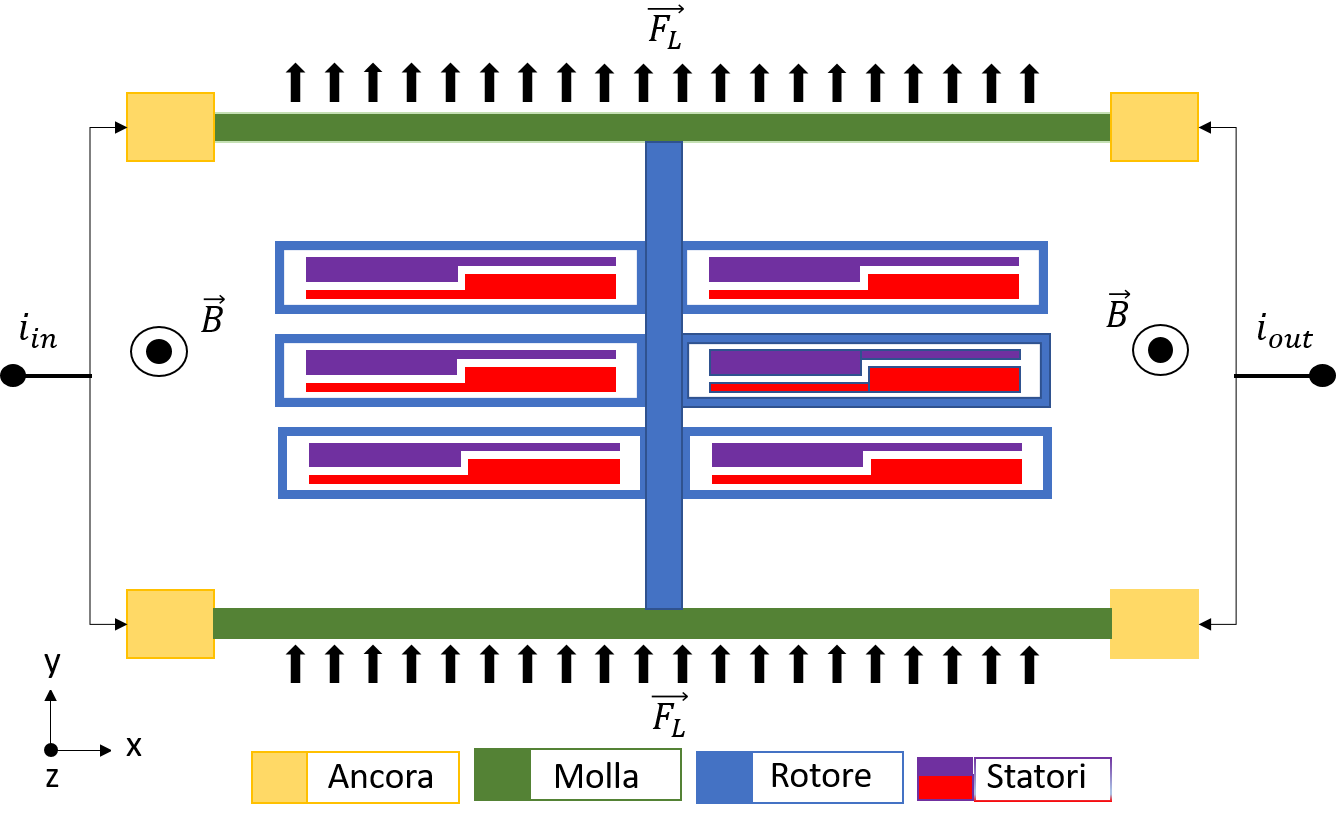
\includegraphics[scale=0.4 ]{tecnologie/magnet.png}
	\caption{Rappresentazione esemplificativa di un magnetometro capacitivo lungo l'asse \textit{z}}
	\label{fig:magnet}
\end{figure}


\section{Modello di misura}
\label{modello_di_misura}
Dopo aver introdotto i principi di funzionamento dei sensori è bene specificare il modello di misurazione.\\
I sensori utilizzati hanno tre assi lungo i quali una \textit{"quantità fisica"} (esempio forza, velocità angolare, campo magnetico) è convertita in un segnale di tensione in uscita. \\
Tipicamente questi sensori hanno un comportamento lineare nell'area di lavoro. Sulla base di questa osservazione, la seguente equazione (semplificata) descrive la relazione tra la forza fisica $y(t)$ e la tensione in uscita dal sensore $ u(t)$:

\begin{equation}
    u(t) = G R y(t) + c
\end{equation}
Dove:
\begin{itemize}
	\item $G$ è la matrice diagonale contenente il guadagno per ogni asse sensibile
	\item $R$ è la matrice di allineamento che specifica la direzione degli assi
	\item $c$ è il vettore di offset 
\end{itemize}
Al fine di discutere il modello di misura, si devono introdurre i seguenti sistemi di coordinate (in inglese: coordinate frames) rappresentati in Fig.\ref{fig:frames}:

\begin{itemize}
	\item Il \textbf{frame del corpo} - \textit{b-frame} (in inglese: \textit{body frame}): è il sistema							 di riferimento dei movimenti dell'IMU. L'origine è posta al centro dei sensori e allineata al case posto sul chip. Tutte le misure inerziali sono calcolate su questo sistema di riferimento.
	\item Il \textbf{frame di navigazione} - \textit{n-frame} (in inglese: \textit{navigation frame}) è il frame geografico nel quale vogliamo navigare. Per navigazioni a corto raggio è considerato statico rispetto alla terra.
	\item Il \textbf{frame inerziale} - \textit{i-frame} (in inglese: \textit{inertial frame}): è un frame stazionario non rotante. L'IMU misura le forze relativamente a questo frame. La sua origine è posta al centro della terra e i suoi assi sono allineati rispetto alle stelle.
	\item Il \textbf{frame terrestre} - \textit{e-frame} (in inglese: \textit{earth frame}): coincide con l' i-frame ma ruota intorno alla terra. L'origine è posta al centro della terra e gli assi fissati rispetto ad essa.
\end{itemize}



\begin{figure}[H]
	\centering    
	\label{fig:frames}
	\subfigure[]{\label{fig:framesa}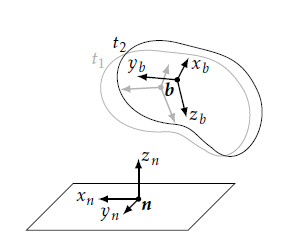
\includegraphics[width=60mm]{tecnologie/framesa.png}}
	\subfigure[]{\label{fig:framesb}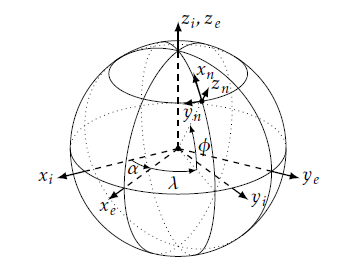
\includegraphics[width=60mm]{tecnologie/framesb.png}}
	\caption{in \ref{fig:framesa} il \textit{b-frame} nell'istante $t_1$ e $t_2$ relativamente al \textit{n-frame}, in \ref{fig:framesb} l'\textit{n-frame} in latitudine $\varphi$ e longitudine $\lambda$, l'\textit{e-frame} all'angolo $\alpha(t)= \omega_{ie}t$ e l'\textit{i-frame}}
\end{figure}
Ignorando la dipendenza dal tempo delle quantità coinvolte, la misura del giroscopio (si veda \ref{giroscopi}) è modellata in \cite{gyromodel} come:

\begin{equation}
y_\omega = \omega_{ib}^b + \delta_{\omega}^b + e_\omega^b
\end{equation}

Dove:
\begin{itemize}
	\item $\omega_{ib}$ è la velocità angolare nel \textit{b-frame} osservata dall'\textit{i-frame}
	\item $\delta_\omega$ è la deriva del sensore che varia lentamente nel tempo 
	\item $e_w^b$ è il rumore gaussiano
\end{itemize}

La velocità angolare $\omega_{ib}$ può essere così estesa:

\begin{equation}
\omega_{ib} = R^{bn} ( \omega_{ie}^n + \omega_{en}^n) + \omega_{nb}^b
\end{equation}

Dove:
\begin{itemize}
	\item $ R$ è la matrice di rotazione
	\item $\omega_{ie}$ è la velocità angolare della terra
	\item $\omega_{en}$ è velocità angolare di transporto
	\item $\omega_{nb}$ è la velocità angolare richiesta ai fini della navigazione
\end{itemize}

La misura dell'accelerometro $y_a$ è invece modellata in \cite{gyromodel} come:

\begin{equation}
\label{accelModel}
 y_a = f^b + \delta_a^b + e_a^b = R^{bn} (\ddot{b}_{ii}^n - g^n) + \delta_a^b + e_a^b
\end{equation}
Dove:
\begin{itemize}
	\item $f$ è la specifica forza esterna
	\item $\delta_a$ è la deriva del sensore che varia lentamente nel tempo 
	\item $e_a$ è il rumore gaussiano
\end{itemize}
L'Eq.\ref{accelModel} divide la forza specifica nei suoi contributi provenienti dall'accelerazione lineare del corpo osservata dall'\textit{i-frame} ($\ddot{b}_{ii}$) e dal vettore gravitazione $g$. L'accelerazione lineare può a sua volta essere espansa come:

\begin{equation}
\ddot{b}_{ii} = \omega_{ie}^n \times \omega_{ie}^n \times R^{ni}b^i + 2\omega_{ie}^n \times \dot{b_n^n}+\ddot{b_{nn}^n}
\end{equation}

dove $\ddot{b_{nn}}$ è l'accelerazione del corpo osservata dal \textit{n-frame} richiesto per la navigazione.\\

Infine per il magnetometro (si veda \ref{magnetometro}) la misura $y_m$ è così modellata:

\begin{equation}
y_m = m^b + e_b^b = R^{bn} m^n + e_m^b
\end{equation}
Dove:
\begin{itemize}
	\item $m$ è il vettore del campo magnetico locale
	\item $e_m$ è il rumore gaussiano
\end{itemize}
In assenza di oggetti ferromagnetici, $m$ è il campo magnetico della terra e la misura del magnetometro può essere usata come una bussola per trovare la direzione del nord magnetico.








\chapter{Stima dell'assetto tramite sensor fusion (NON completo)}
\label{elaborazione}
In questo capitolo vengono inizialmente illustrati gli strumenti matematici utilizzati per rappresentare l'assetto di un corpo rigido nello spazio,
successivamente viene illustrato l'algoritmo di fusione dei dati, provenienti dall'unità di misura inerziale, utilizzato per la stima dell'assetto dell'operatore.


\section{Rappresentazione geometrica dell'assetto di un corpo rigido nello spazio}
\label{assetto}
Con \textit{"assetto di un corpo rigido"} si intende l'orientamento di un corpo rigido rispetto ad un particolare sistema di riferimento.\\
Tale orientamento è rappresentato da una matrice di rotazione che, applicata ad un qualsiasi vettore nel sistema di riferimento mobile, ne fornisce una rappresentazione nel sistema di riferimento fisso (\ref{modello_di_misura}). 
Tale rotazione può essere espressa attraverso numerosi strumenti matematici, tra i più utilizzati si hanno:
\begin{itemize}
	\item \textbf{Angoli di Eulero}
	\item \textbf{Quaternioni unitari}
\end{itemize}

Nella Tab.\ref{rappresentazioni} vengono riportate sinteticamente le caratteristiche delle rappresentazioni appena enunciate \cite{assetto}:

\begin{table}[H]
	\centering

	\label{rappresentazioni}
	\begin{tabular}{lllll}
		\cline{1-3}
		\multicolumn{1}{|l|}{\textbf{Rappresentazione}} & \multicolumn{1}{l|}{\textbf{\#Parametri}} & \multicolumn{1}{l|}{\textbf{Caratteristiche}}                                                                                                                                                                                                                                                    &  &  \\ \cline{1-3}
		\multicolumn{1}{|l|}{Angoli di Eulero}          & \multicolumn{1}{c|}{3}                    & \multicolumn{1}{l|}{\begin{tabular}[c]{@{}l@{}}- facilmente interpretabili \\ dall'essere umano\\ \\ - funzioni trigonometriche nelle \\ relazioni cinematiche\\ \\ -soffrono del fenomeno \\ noto come \textit{Gimbal lock}\\ \\ - meno accurati dei quaternioni\end{tabular}}                           &  &  \\ \cline{1-3}
		\multicolumn{1}{|l|}{Quaternioni unitari}       & \multicolumn{1}{c|}{4}                    & \multicolumn{1}{l|}{\begin{tabular}[c]{@{}l@{}}- non interpretabili facilmente\\ dall'essere umano\\ \\ - equazioni della cinematica \\ lineari\\ \\ - costo computazione di \\ elaborazione minore degli\\ angoli di Eulero\\ \\ - necessitano di un vincolo di \\ norma unitaria\end{tabular}} &  &  \\ \cline{1-3}
		&                                           &                                                                                                                                                                                                                                                                                                  &  & 
	\end{tabular}
	\caption{Tabella comparativa delle rappresentazioni d’assetto}
\end{table}
Nell'algoritmo di fusione dei dati, dettagliato nei paragrafi successivi, si è adottato un approccio ibrido molto comune nei contesti applicativi dei sistemi IPS(\ref{IPS}). Tale approccio consiste nell'utilizzare la rappresentazione mediante \textit{quaternioni} per le computazioni mentre la rappresentazione mediante gli \textit{angoli di Eulero} per la visualizzazione.\\

\subsection{Matrice di rotazione}
Di seguito si fornisce una definizione generale di matrice di assetto\cite{assetto2}. Si supponga di avere due sistemi di riferimento cartesiani in tre dimensioni $F$ e $G$, una matrice ortogonale $A_{FG}$, detta di rotazione ed un vettore $x_G$ espresso nel sistema di riferimento $G$.\\
La matrice $A_{FG}$ permette di esprimere il vettore $x_G$ rispetto al sistema di riferimento $F$ secondo la seguente equazione:

\begin{equation}
x_F = A_{FG}x_G
\end{equation}
Essendo per ipotesi la matrice $A_{FG}$ ortogonale, l'operazione di inversione corrisponde al calcolo della sua trasposta:
 \begin{equation}
 x_G = A_{FG}^Tx_F
 \end{equation}
 Quindi determinare l'assetto significa definire la matrice di rotazione che permette, attraverso una semplice moltiplicazione, di ruotare i vettori da un sistema di riferimento mobile ad uno fisso.\\
 

\subsection{Angoli di Eulero}
\label{angoliEulero}
Si consideri \cite{assetto2} un sistema di riferimento cartesiano $F$  fisso (con assi $x_F$,$y_F$ e $z_F$) ed un sistema di riferimento cartesiano $G$ mobile (con assi $x_G$,$y_G$ e $z_G$). \\
Affinché l'orientamento degli assi del sistema mobile $G$ coincida con quelli del sistema fisso $F$, si devono eseguire almeno tre rotazioni successive attorno ai tre assi.\\
Tale vincolo è posto dal teorema di Eulero che è alla base di tutte le matrici di rotazioni. Il teorema afferma che:
\begin{itemize}
	\item Per ogni rotazione, esiste sempre un vettore che avrà la medesima rappresentazione nei due sistemi di riferimento
	\item ogni rotazione avviene sempre attorno ad un asse fisso
\end{itemize} 
L'idea è quella di ruotare ogni volta il sistema attorno ad uno dei suoi tre assi, così facendo l'asse attorno al quale è avvenuta la rotazione rimane fisso, mentre gli altri due cambiano orientamento. La rotazione successiva verrà fatta attorno ad uno dei due precedenti assi che hanno mutato l'orientamento. Con sistemi cartesiani a tre assi è possibile quindi scegliere tra dodici differenti sequenze di rotazioni per un totale eguale di possibili rappresentazioni della matrice di rotazione.\\
Nell'ambito di questa tesi e più comunemente in quello aeronautico, si è utilizzata la sequenza di rotazioni $z$-$y$-$x$ e gli angoli $\psi$,$\vartheta$ e $\varphi$ chiamati rispettivamente \textit{imbardata,beccheggio e rollio} (in inglese \textit{yaw,pitch e roll}) mostrati in Fig.\ref{fig:rpy}:
\begin{figure}[H]  
	\centering 
	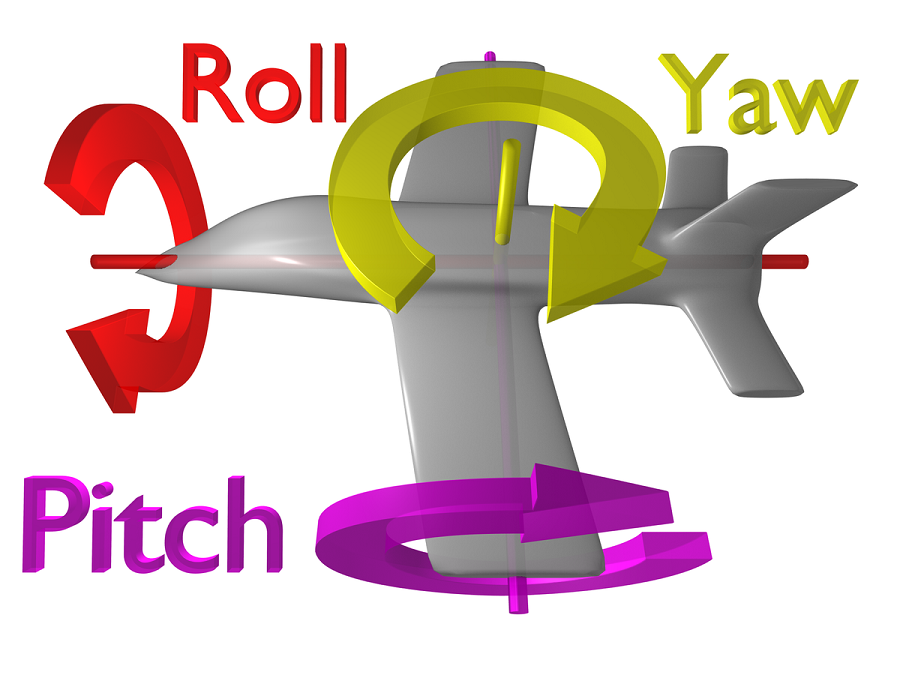
\includegraphics[scale=0.5]{elaborazione/rpy.png}
	\caption{Rappresentazione degli angoli di roll, pitch e yaw per un velivolo \cite{wikiRoll}}
	\label{fig:rpy}
\end{figure}
Le tre rotazioni in questione sono:

\begin{equation}
A(z,\psi)= \begin{bmatrix}
\cos\psi   &-\sin\psi & 0 \\
\sin\psi     & \cos\psi  & 0 \\
0      & 0 & 1
\end{bmatrix}
\end{equation}

\begin{equation}
A(y,\vartheta)= \begin{bmatrix}
\cos\vartheta   &0 & \sin\vartheta \\
0    & 1  & 0 \\
-\sin\vartheta     & 0 & \cos\vartheta
\end{bmatrix}
\end{equation}


\begin{equation}
A(x,\varphi)= \begin{bmatrix}
1   &0 & 0 \\
0    & \cos\varphi  & -\sin\varphi\\
0     & \sin\varphi & \cos\varphi
\end{bmatrix}
\end{equation}

Andando a moltiplicare le precedenti matrici si ottiene la matrice di rotazione cercata:

\begin{eqnarray}
\label{matriceRotazione}
A(\psi,\vartheta,\varphi)= \begin{bmatrix}
\cos\psi \cos\vartheta  & \cos\psi \sin\vartheta \sin\varphi-\sin\psi \cos\varphi & \cos\psi \sin\vartheta \cos\varphi + \sin\psi \sin\varphi \\
\sin\psi \cos\vartheta    & \sin\psi \sin\vartheta \sin\varphi+\cos\psi \cos\varphi & \sin\psi \sin\vartheta \sin\varphi - \cos\psi \sin\varphi\\
-\sin\vartheta    & \cos\vartheta\sin\varphi & \cos\vartheta\cos\varphi
\end{bmatrix}
\end{eqnarray}

Il significato geometrico si ha osservando la Fig.\ref{fig:eulero}, dove:
\begin{itemize}
	\item la linea dei nodi è definita come l'intersezione tra il piano individuato dagli assi $x_Fy_F$ e quello individuato dagli assi $y_Bz_B$
	\item $\psi$ è l'angolo tra $y_F$ e la linea dei nodi
	\item $\vartheta$ è l'angolo tra $x_B$ e la sua proiezione sul piano $x_Fy_F$
	\item $\varphi$ è l'angolo tra $y_B$ e la linea dei nodi
\end{itemize}

\begin{figure}[H]  
	\centering 
	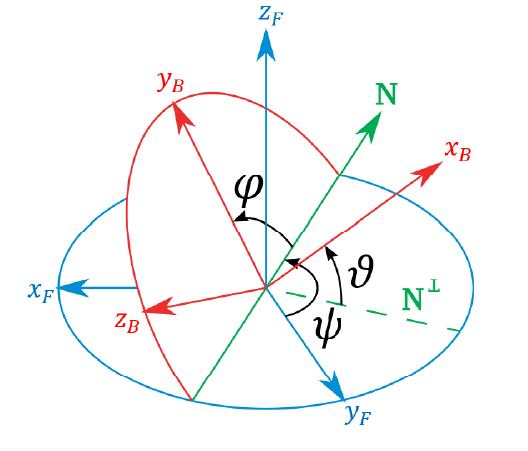
\includegraphics[scale=0.8]{elaborazione/eulero.png}
	\caption{Significato geometrico degli angoli di Eulero \cite{assetto2}}
	\label{fig:eulero}
\end{figure}
Come accennato nella tabella \ref{rappresentazioni}, la rappresentazione dell'assetto mediante angoli di Eulero presenta un problema di singolarità noto come \textit{gimbal lock}.\\
Nel caso della matrice di rotazione ricavata nell'equazione \ref{matriceRotazione}, il problema si presenta per $\vartheta = \pm \dfrac{\pi}{2}$: in questa situazione esistono infinite combinazioni di $\varphi$ e $\psi$ che portano alla stessa matrice di rotazione, nel caso di $\vartheta= \dfrac{\pi}{2}$ si ha:
\begin{equation}
\label{matriceGimbal}
A(\psi,\vartheta,\varphi)= \begin{bmatrix}
0   &\sin(\varphi - \psi) & \cos(\varphi - \psi) \\
0    & \cos(\varphi-\psi)  &-\sin(\varphi - \psi)\\
-1    & 0 & 0
\end{bmatrix}
\end{equation}
Ottenuta mediante sostituzione e applicazione delle formule di addizione e sottrazione di seno e coseno. Mentre la matrice di rotazione in Eq.\ref{matriceRotazione} permette una rotazione completa attorno ad un qualsiasi asse, la matrice in \ref{matriceGimbal} permette la rotazione attorno al solo asse $X$. Quindi si manifesta un vincolo di rotazione con conseguente perdita di un grado di libertà, come mostrato in Fig.\ref{fig:gimbal}. \\
Basti pensare ad un velivolo con un \textit{pitch} di $90°$, modificare il \textit{roll} o lo \textit{yaw} di un certo angolo avrebbe il medesimo effetto.\\
\begin{figure}[H]  
	\centering 
	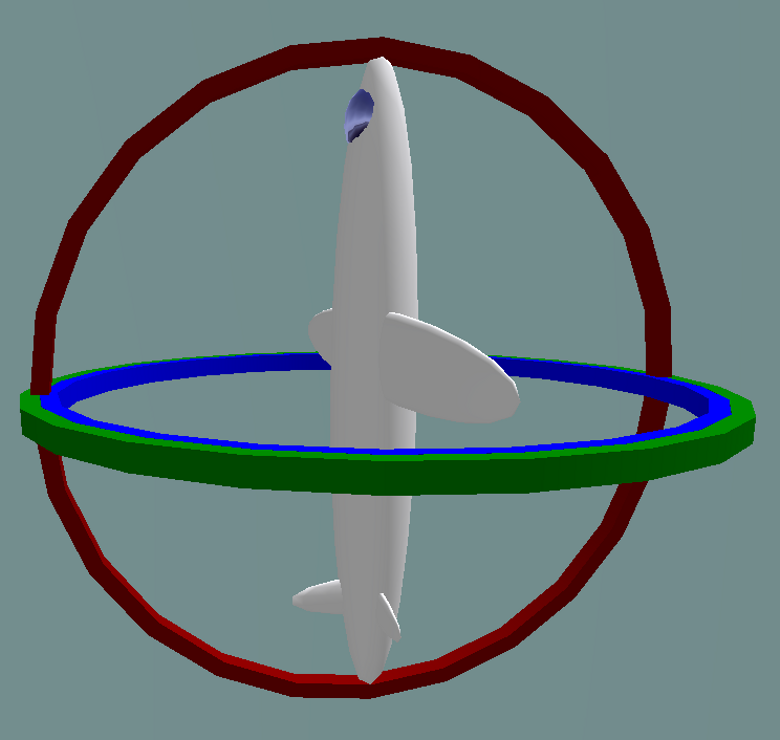
\includegraphics[scale=0.3]{elaborazione/gimbal.png}
	\caption{Rappresentazione del fenomeno di \textit{gimbal lock} \cite{gimbal}}
	\label{fig:gimbal}
\end{figure}



\subsection{Quaternioni unitari}
\label{quaternioni}
I quaternioni hanno la peculiarità di essere il metodo di rappresentazione dell'assetto con minor numero di parametri privi di singolarità, come ad esempio il \textit{gimbal lock} visto precedentemente per gli angoli di Eulero.\\
Il quaternione unitario è un vettore composto da tre elementi che definiscono il vettore \textbf{$q_{1:3}$} e da un elemento scalare $q_4$, tale che la norma:
\begin{equation}
 ||\overrightarrow{q}|| = \sqrt{q_1^2 + q_2^2 + q_3^2 + q_4^2}=1
\end{equation}
Questi possono essere usati per rappresentare l'assetto di un corpo rigido in quanto le trasformazioni che legano le terne di Eulero ai quaternioni unitari, sono semplicemente delle trasformazioni algebriche che portano da uno spazio rappresentativo all'altro.\\
Sfruttando il teorema di Eulero \cite{assetto2}, si può parametrizzare la matrice di rotazione in \ref{matriceRotazione} ottenendo l'equivalente in funzione dei quaternioni:
\begin{equation}
\label{matriceQuaternioni}
A(\overrightarrow{q})= \begin{bmatrix}
 q_1^2 -  q_2^2 -  q_3^2 -  q_4^2 & 2(q_1 q_2 + q_3  q_4) & 2(q_1 q_3 - q_2 q_4) \\
2(q_2 q_1 - q_3 q_4)    &  -q_1^2 + q_2^2 -  q_3^2 +  q_4^2  & 2(q_2 q_3 + q_1q_4)\\
2(q_3 q_1 + q_2 q_4)    & 2(q_3 q_2 - q_1 q_4)  &  -q_1^2 -  q_2^2 +  q_3^2 +  q_4^2
\end{bmatrix}
\end{equation}
Come si può notare dalla \ref{matriceRotazione}, i quaternioni permettono di definire una matrice di assetto i cui elementi sono funzioni quadratiche omogenee degli elementi del quaternione. Si evita così qualsiasi tipo di calcolo trigonometrico (e relative singolarità) e si ha un costo computazionale minore.\\

Un diretto confronto tra le matrici \ref{matriceRotazione} e \ref{matriceQuaternioni} permette inoltre di definire il rapporto tra gli angoli di Eulero ($\psi,\vartheta,\varphi$) e le componenti del quaternione ($q_1, q_2, q_3,q_4$) attraverso le seguenti:

\begin{equation}
\psi = Atan2 \left( \frac{2q_2q_3 - 2q_1q_4}{2q_1^2+q_2^2 -1}\right)
\end{equation}

\begin{equation}
\vartheta = -\sin(2q_2q_4 + 2q_1q_3)
\end{equation}

\begin{equation}
\psi = Atan2\left(  \frac{2q_3 q_4 - 2q_1q_2}{2q_1^2+q_4^2 -1}\right)
\end{equation}


\section{Algoritmo di sensor fusion per la stima dell'assetto}
\label{sensor_fusion}
La maggior parte degli algoritmi di stima dell'assetto che sfruttano i dati provenienti da sensori (sez.\ref{tecnologie}) si basano sull'applicazione di un \textit{filtro di Kalman}.\\
Il filtro di Kalman è un efficiente filtro ricorsivo che valuta lo stato di un sistema dinamico a partire da una serie di misure soggette a rumore. Per le sue caratteristiche intrinseche è un filtro ottimo per rumori e disturbi agenti su sistemi gaussiani a media nulla \cite{kalmanWiki}.\\
Con riferimento alla rappresentazione del sistema realizzato nell'ambito di questa tesi (sez.\ref{livello_moduli}), all'interno del "modulo" \textit{microcontroller} e del "modulo" \textit{App} vi sono due diversi algoritmi di \textit{sensor fusion} basati sul filtro di Kalman che, a partire dai dati grezzi letti dall'unità di misura inerziale (sez.\ref{tecnologie}), stimano l'assetto relativo al modello di misura (sez.\ref{modello_di_misura}).\\
Il modulo \textit{Microcontroller} utilizza una libreria esterna realizzata da \textit{STM} \cite{motion} della quale però non vengono forniti i dettagli implementativi, perciò nei paragrafi successivi si farà riferimento all'algoritmo utilizzato all'interno del modulo \textit{App} che è  l'implementazione di un lavoro di tesi trovato in letteratura \cite{trackingThesis}.

\subsection{Equazioni di stato del sistema}

 E' necessario come prima cosa, descrive l'evoluzione del sistema con un equazione differenziale, dove lo stato del sistema è rappresentato tramite quaternioni unitari (\ref{quaternioni}).\\
 Definiamo con $\omega_{nb}^n$ il vettore delle velocità angolari rispetto al \textit{b-frame} dell'IMU (sez.\ref{modello_di_misura}):
 
\begin{equation}
\label{vettoreAngular}
\omega_{nb}^b  = [\omega_x, \omega_y, \omega_z]^T
\end{equation}

Dall'algebra dei quaternioni è possibile scrivere l'equazione che descrive l'evoluzione del sistema come:

\begin{equation}
\label{stateEquation}
\dot{q}_{n}^b = \frac{1}{2} \Omega_{nb}^n q_n^b
\end{equation}
Dove $\Omega_{nb}^n$ è la matrice con gli elementi del vettore della velocità angolare in \ref{vettoreAngular}:
\begin{equation}
\Omega_{nb}^n= \begin{bmatrix}
0 &  -\omega_x &  -\omega_y & -\omega_z\\
\omega_x     & 0  & \omega_z &  -\omega_y  \\
 \omega_y & -\omega_z  & 0 &  \omega_x \\
 \omega_z & \omega_y & -\omega_x & 0
\end{bmatrix}
\end{equation}

Si noti bene come dalla precedente equazione \ref{stateEquation} l'evoluzione del sistema, corrispondente alla fase detta "aggiornamento a priori" del filtro di Kalman, è caratterizzata dai soli dati del giroscopio. Come si vedrà tra poco, i sensori di accelerometro (sez.\ref{accell}) e magnetometro (sez.\ref{magnetometro}) verranno utilizzati nella fase detta "aggiornamento a posteriori" per correggere la stima ottenuta con il solo giroscopio.

\subsection{Filtro di Kalman a due stadi}
Un filtro di Kalman completo potrebbe essere computazionalmente troppo oneroso da eseguire per un dispositivo come un microcontrollore. Per questo motivo in \cite{trackingThesis} si è pensato di adottare un approccio diverso dall'implementazione classica del filtro. Tale metodo è ancora basato sul filtro di Kalman, ma la fase di correzione della stima ottenuta nell'aggiornamento a priori, viene divisa in due parti, ognuna delle quali agisce su una specifica componente.\\
Il primo stadio utilizza i dati provenienti dall'accelerometro (sez.\ref{accell}) per correggere gli angoli stimati di \textit{roll} e \textit{pitch} (sez.\ref{angoliEulero}) mentre il secondo stadio utilizza i dati provenienti dal magnetometro (sez.\ref{magnetometro}) per correggere la stima dello \textit{yaw}. Ogni stadio lavora con un singolo vettore di dati grezzi che è usato appunto per correggere una specifica parte della stima dell'assetto, da questo ne consegue che ogni stadio può lavorare con una matrice di dimensione $ 4 x 3$ contro le $ 4 x 6$ di un filtro di Kalman completo. Da questo ne consegue un guadagno notevole in termini di prestazioni.\\
 Nella figura seguente una rappresentazione a blocchi del filtro a due stadi:
\begin{figure}[H]  
	\centering 
	
\includegraphics[scale=0.3]{elaborazione/filtro.png}
	\caption{Rappresentazione del principio di funzionamento del filtro di Kalman a due stadi \cite{trackingThesis}}
	\label{fig:filtro}
\end{figure}

Un altro grande vantaggio consiste nella flessibilità dell'algoritmo, questo infatti può essere utilizzato anche se si dispone di un IMU a 6DOF (privo del magnetometro) semplicemente "disattivando" lo \textit{stadio 2} in Fig.\ref{fig:filtro}, così facendo l'uscita dallo \textit{stadio 1} diventa l'uscita del sistema e viene retroazionata allo \textit{stadio 0} andando a correggere la prossima lettura.
 
\subsection{Descrizione dell'algoritmo}
\label{descrizioneAlgoritmo}
Lo stato del sistema è, come già detto, rappresentato tramite quaternioni (sez.\ref{quaternioni}). Lo \textit{stadio 0} anche detto \textit{stima a priori} utilizza solo i dati grezzi provenienti dal giroscopio.
Fatto ciò, si deve stimare il vettore gravitazionale $h_1$ per poter correggere il \textit{roll} e il \textit{pitch} nello \textit{stadio 1}. Tale vettore è così definito:
\begin{eqnarray}
h_1(q_k)= \hat{q}= R_n^b \begin{bmatrix}
0  \\
0 \\
|q|
\end{bmatrix}= |g| \begin{bmatrix}
2q_2q_4 - 2q_1q_3  \\
2q_1q_2 + 2q_3q_4 \\
q_1^2 - q_2^2 - q_3^2 + q_4^3
\end{bmatrix}
\end{eqnarray}
Il vettore gravitazionale $g$, espresso secondo l'\textit{i-frame} (sez.\ref{modello_di_misura}), viene riportato nel \textit{b-frame} utilizzando la seguente matrice di rotazione:
\begin{equation}
R_n^b= \begin{bmatrix}
q_1^2 +  q_2^2 -  q_3^2 -  q_4^2 & 2(q_2 q_3 + q_1  q_4) & 2(q_2 q_4 - q_1 q_3) \\
2(q_2 q_3 - q_1 q_4)    &  q_1^2 - q_2^2 +  q_3^2 -  q_4^2  & 2(q_3 q_4 + q_1q_2)\\
2(q_2 q_4 + q_1 q_3)    & 2(q_3 q_4 - q_1 q_2)  &  q_1^2 -  q_2^2 - q_3^2 +  q_4^2
\end{bmatrix}
\end{equation}
Da $h_1$ si ricava quindi la matrice $H_{k1}$ del guadagno di Kalman che verrà utilizzata successivamente dallo \textit{stadio 1}:
\begin{eqnarray}
H_{k1}= \frac{\delta h_{1[i]}}{\delta q_j}=  \begin{bmatrix}
-2q_3 & 2q_4 & -2q_1 & 2q_2  \\
2q_2 & 2q_1 & 2q_4 & 2q_3\\
2q_1 & -2q_2 & -2q_3 & 2q_4
\end{bmatrix}
\end{eqnarray}  
Lo \textit{stadio 1} calcola il residuo $q_{\epsilon 1}$ che sarà sommato allo stato $\hat{x_k}$, stimato a \textit{priori} dallo \textit{stadio 0}, ottenendo così la prima stima a \textit{posteriori} $\hat{x_{k1}}$. L'elemento $q_{\in1,4}$ è posto a zero, al fine di essere sicuri che lo \textit{stadio 1} corregga solo \textit{roll} e \textit{pitch}. Il residuo $q_{\epsilon 1}$ è determinato dalla seguente relazione:

\begin{equation}
q_{\epsilon 1}= K_{k1}(z_{k1}-h_1(\hat{x_k},0))= q_{\in1,1} + q_{\in1,2} + q_{\in1,3} + 0 \cdot q_{\in1,4} 
\end{equation}

e quindi la stima dello stato a \textit{posteriori} risulta:
\begin{equation}
\hat{x_{k1}} = \hat{x}_k + q_{\epsilon 1}
\end{equation}

Per lo \textit{stadio 2} è necessario stimare il vettore del campo magnetico $h_2$:

\begin{equation}
h_2(q_k) = \hat{m} = R_n^b \begin{bmatrix}
0 \\
1 \\
0
\end{bmatrix} = 
\begin{bmatrix}
2q_2q_3 + 2q_1q_4 \\
q_1^2 - q_2^2 - q_3^2 - q_4^2 \\
2q_3q_4 - 2q_1q_2
\end{bmatrix} 
\end{equation}

La matrice $H_{k2}$ usata dallo \textit{stadio 2} per calcolare il guadagno di Kalman è la seguente:
\begin{eqnarray}
H_{k2}= \frac{\delta h_{2[i]}}{\delta q_j}=  \begin{bmatrix}
2q_4 & 2q_3 & 2q_2 & 2q_1  \\
2q_1 & -2q_2 & -2q_3 & -2q_4\\
-2q_2 & -2q_1 & -2q_4 & 2q_3
\end{bmatrix}
\end{eqnarray}  
Si ottiene così il secondo residuo $q_{\in 2}$ che verrà sommato alla precedente stima a \textit{posteriori} determinata dallo \textit{stadio 1}. In questo caso, al fine di essere sicuri che lo \textit{stadio 2} corregga solo lo \textit{yaw}, le componenti del residuo poste a zero sono $q_{\in 2,2}$ e $q_{\in 2,3}$ :

\begin{equation}
q_{\epsilon 2}= q_{\in2,1} + 0 \cdot q_{\in2,2} + 0 \cdot q_{\in2,3} + q_{\in2,4} 
\end{equation}

E infine l'ultima stima a \textit{posteriori} è data da:

\begin{equation}
\hat{x_{k}} = \hat{x}_{k1} + q_{\epsilon 2}
\end{equation}


\subsection{Trasformazione del sistema a tempo discreto}
L'equazione precedenti descrivono l'evoluzione del sistema nel dominio del tempo continuo. Per implementare tale filtro si devono trasformare l'equazioni in \ref{descrizioneAlgoritmo} nel dominio del tempo discreto. \\
In \cite{trackingThesis} si utilizzano le formule standard per discretizzare un sistema a tempo continuo in uno a tempo discreto. Il sistema di partenza è descritto da un'equazione del tipo:
\begin{equation}
\label{sistemaContinuo}
\dot{x}= A_{TC} x(t) + B_{TC} u(t)
\end{equation}

dove $A_{TC}$ e $B_{TC}$ sono le matrici di stato e d'ingresso mentre $x(t)$ e $u(t)$ sono le variabili di stato e dell'ingresso nel tempo continuo.\\
Dalla definizione di derivata si ottiene la seguente relazione:
\begin{equation}
\dot{x} = \lim\limits_{x\rightarrow0} \dfrac{x(t+T)-x(t)}{T} = A_{TC}x(t) + B_{TC}u(t)
\end{equation}

La variabile $T$ è il \textit{delta-time} trascorso tra ogni iterazione in un sistema digitale, quindi è possibile rimuovere l'operazione di limite ed ottenere:
\begin{equation}
x(t+T)=x(t)+ A_{TC}x(t)T + B_{TC}u(t)T = (I + A_{TC}T)x(t) + B_{TC}Tu(t)
\end{equation}
In conclusione il sistema a tempo continuo di partenza nell'equazione \ref{sistemaContinuo} si trasforma nel seguente sistema a tempo discreto:
\begin{equation}
x_k = A x_{k-1} + B u_k
\end{equation}
Dove $x_k$ è equivalente alla variabile $x(t)$ campionata all'istante $t + T$ e:
\begin{equation}
A = I + A_{TC}T
\end{equation}

\begin{equation}
B = B_{TC}T
\end{equation}

\subsection{Riepilogo algoritmo step-by-step}
Per maggiore chiarezza,di seguito si fornisce un riepilogo dell'algoritmo step-by-step:
\begin{itemize}
	\item Calcolo della matrice di transizione dello stato discreta $A_k= I + \frac{1}{2} \Omega_{nb}^n T$
	\item Calcolo della stima a \textit{priori} dello stato mediante lo \textit{stadio 0},  $\hat{q}_k = A_k\hat{q}_{k-1}$
	\item Calcolo della matrice di covarianza del rumore  $P_k = A_kP_{k-1}A_k^T + Q_k$
\end{itemize}

\textit{Inizio della correzione mediante lo stadio 1}
\begin{itemize}
\item Calcolo della matrice $H_{k1} = \begin{bmatrix}
-2q_3 & 2q_4 & -2q_1 & 2q_2  \\
2q_2 & 2q_1 & 2q_4 & 2q_3\\
2q_1 & -2q_2 & -2q_3 & 2q_4
\end{bmatrix}$
\item Calcolo del guadagno di Kalman $K_{k1} = P_k H_{k1}^T ( H_{k1} P_k H_{k1}^T + V_{k1}R_{k1}V_{k1}^T)^{-1}$
\item Calcolo di $h_1(\hat{q}_k) = \begin{bmatrix}
2q_2q_4 - 2q_1q_3  \\
2q_1q_2 + 2q_3q_4 \\
q_1^2 - q_2^2 - q_3^2 + q_4^3
\end{bmatrix} $
\item Calcolo del fattore di correzione  $q_{\in 1} = K_{k1}(z_{k1}-h_1(\hat{q}_k)) con q_{\in1,4} =0$ e dove $z_{k1}$ corrisponde alle accelerazioni sui tre assi lette dall'accelerometro.
\item Calcolo della prima stima dello stato a \textit{posteriori}  $\hat{q}_{k1}= \hat{q}_k + q_{\in1}$
\item Calcolo della matrice di covarianza del rumore a \textit{posteriori} $P_{k1} = ( I - K_{k1}H_{k1})P_k$
\end{itemize}
\textit{Inizio della correzione mediante lo stadio 2}
































\input{Implementazione}
\chapter{Analisi e validazione dei risultati}
\label{analisi}

\section{Analisi temporale}
\label{analisiTemporale}
Questo tipo di analisi è stata effettuata al fine di determinare la frequenza massima entro la quale il microcontrollore è in grado di eseguire tutte le operazioni basilari, rappresentate in Fig.\ref{fig:op}. Ovvero per rispondere alla seguente domanda:
\begin{quotation}
	\textit{Qual'è la finestra temporale minima sufficiente a garantire 
		che il microcontrollore sia in grado di eseguire correttamente le funzioni basilari? }
\end{quotation}
Dove per funzioni basilari si intendono le operazioni di:
\begin{itemize}
	\item \textbf{Lettura} dei dati grezzi dall'IMU tramite, indicato con $T_{RX\_I2C}$
	\item \textbf{Elaborazione} dei dati grezzi (solo per le modalità \textit{HCM} e \textit{TCM}), indicato con $T_{MotionFX}$
	\item \textbf{Trasmissione} dei dati verso il modulo \textit{App} (si veda\ref{livello_moduli}), indicato con $T_{TX\_USB}$
\end{itemize}


\begin{figure}[H]
	\centering
	\label{fig:op}    
	\subfigure[]{\label{fig:op1}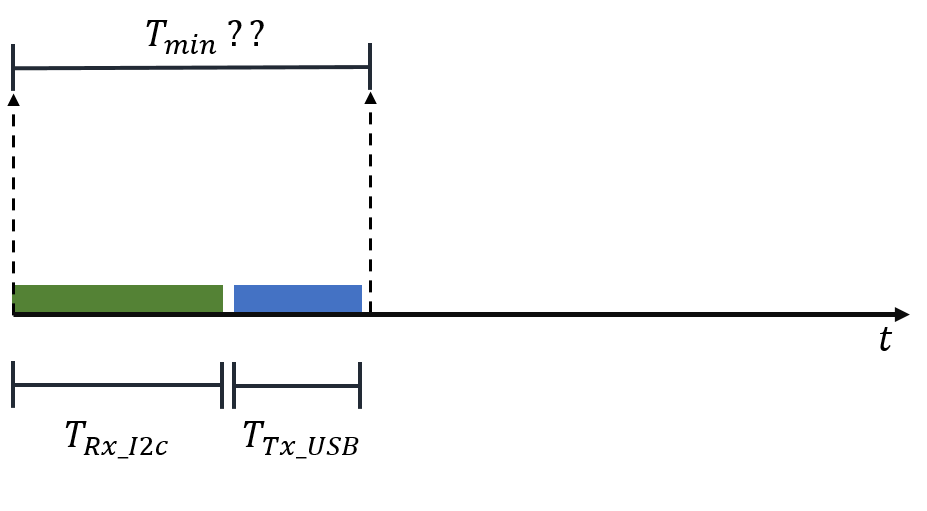
\includegraphics[width=60mm]{analisi/op1.png}}
	\subfigure[]{\label{fig:op2}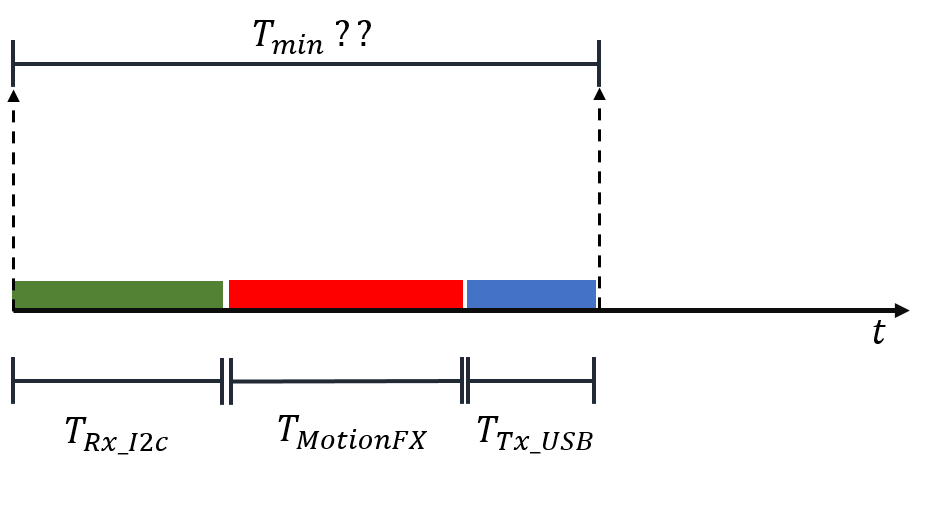
\includegraphics[width=60mm]{analisi/op2.png}}
	\caption{In \ref{fig:op1} le operazioni basilari per la modalità \textbf{LCM}, in \ref{fig:op2} le operazioni basilari per le modalità \textbf{HCM} e \textbf{TCM}}
\end{figure}

Per far ciò è opportuno analizzare singolarmente i due tempi, considerando le relative informazioni e la velocità del mezzo di comunicazione.\\

\subsection{Analisi del tempo di lettura dei dati grezzi dall'IMU}
\label{analisii2c}
Le informazioni riguardanti le grandezze fisiche misurate dai sensori integrati nell'IMU (Cap.\ref{tecnologie}), tramite I2C (Cap.\ref{imp_i2c}), su un singolo asse del \textit{b-frame} (Cap.\ref{modello_di_misura}), sono rappresentate attraverso \textbf{16 bit}.\\
Di conseguenza il tempo di lettura $T_{RX\_I2C}$ è dato dalla seguene equazione:
\begin{equation}
\label{eq:ti2c}
	T_{RX\_I2C} = N_{sensori} \cdot N_{assi} \cdot T_{i\_asse}
\end{equation}
Dove:
\begin{itemize}
	\item $N_{sensori}$ sono il numero di sensori utilizzati 
	\item $N_{assi}$ sono il numero di assi utilizzati dai sensori
	\item $ T_{i\_asse}$ è il tempo di lettura del singolo asse
\end{itemize}

Dunque il problema si riduce alla determinazione di $ T_{i\_asse}$. Per come è implementata l'IMU, la lettura di un singolo asse si completa leggendo due registri da \textbf{8 bit}.
\begin{equation}
 T_{i\_asse} = 2 \cdot T_{RX\_8bit}
\end{equation}

Per stimare $T_{RX\_8bit}$ si è programmato il microcontrollore in modo tale da leggere 1000 volte un registro da 8 bit e misurare il tempo trascorso leggendo i \textit{tick} di sistema. Per il codice si rimanda alla lettura dell'App.\ref{app:stimai2c}.\\ 
Eseguendo il test svariate volte, si è osservato che il tempo necessario per leggere 1000 volte un registro da 8 bit è pari a $101 ms$. 
Questo implica un \textit{goodput} di $80 Kb/s$ pari al $20\%$ della capacità del canale di comunicazione, che risulta essere $400 Kb/s$ essendo un I2C in \textit{fast-mode}. Questo calo è dovuto a numerosi fattori tra i quali l'overhead del protocollo e la velocità del microcontrollore.\\
Quindi andando a sostituire il valore stimato per la lettura di 8 bit nell'Eq.\ref{eq:ti2c} si ottiene, per l'uso dell'IMU a 9DOF:
\begin{equation}
T_{RX\_I2C} = 3 \cdot 3 \cdot (2 \cdot T_{RX\_8bit}) = 3 \cdot 3 \cdot (2 \cdot 101\mu s )= 1,8 ms
\end{equation}
Mentre per l'uso a 6DOF:
\begin{equation}
T_{RX\_I2C} = 3 \cdot 2 \cdot (2 \cdot T_{RX\_8bit}) = 3 \cdot 2 \cdot (2 \cdot 101\mu s )= 1,2 ms
\end{equation}


\subsection{Analisi del tempo di trasmissione dei dati tramite USB}
\label{analisiusb}
Il tempo necessario per trasmettere un pacchetto, dal modulo \textit{microcontrollore} al modulo \textit{App} (Cap.\ref{livello_sottosistemi}) mediante il canale USB (Cap.\ref{imp_usbcdc}), è dato dalla seguente equazione:
\begin{equation}
\label{tx_usb}
T_{TX\_USB}=  \frac{dim(pack)}{goodput}
\end{equation}
Per stimare il \textit{goodput} si è programmato il microcontrollore in modo da inviare 1000 volte un pacchetto contente un \textit{id} (univoco e incrementale) e un contatore incrementato quando il buffer di trasmissione risulta essere ancora occupato. Per il codice si rimanda alla lettura dell'App.\ref{app:stimausb}.
Eseguendo il test numerose volte, si è osservato che il tempo necessario per trasmettere 1000 pacchetti, per un totale di 8574 Bytes, è di circa $57 ms$. 
Questo implica un \textit{goodput} di $1,2 Mb/s$ pari al $10\%$ della capacità del canale di comunicazione che, essendo un USB 1.1, risulta essere $12 Mb/s$. Ancora una volta questo calo di prestazioni è dovuto a numerosi fattori tra i quali l'overhead del protocollo, l'implementazione della libreria STM utilizzata e la velocità del microcontrollore.\\
Più complicato è il discorso riguardante la dimensione dei pacchetti da trasmettere, questi infatti sono strettamente correlati a:
 \begin{itemize}
 	\item \textbf{La modalità di computazione} selezionata (Cap.\ref{computationMode})
 	\item \textbf{Il numero di sensori} utilizzati
 	\item \textbf{La codifica} dell'informazione
  \end{itemize}

Con riferimento alle possibili combinazioni dei fattori precedenti e alle rispettive strutture dei pacchetti, dettagliate nel Cap.\ref{computationMode}, si hanno le seguenti dimensioni: 
\begin{enumerate}
	\item \textbf{LCM}:
		\begin{enumerate}
		\item \textit{6DOF} = 48 Bytes
		\item \textit{9DOF} = 63 Bytes
		\end{enumerate}
	\item \textbf{HCM} = 21 Bytes
	\item \textbf{TCM}:
			\begin{enumerate}
			\item \textit{6DOF} = 63 Bytes
			\item \textit{9DOF} = 84 Bytes
			\end{enumerate}
\end{enumerate}

Sostituendo questi valori e la stima del \textit{goodput} del canale all'Eq.\ref{tx_usb}, si ottengono le stime dei diversi tempi di trasmissione:

\begin{enumerate}
	\item \textbf{LCM}:
	\begin{enumerate}
		\item \textit{6DOF}: $ T_{TX\_USB}=  \frac{48 Bytes}{1,2 Mbit/s} = 0,32 ms $
		\item \textit{9DOF} : $ T_{TX\_USB}=  \frac{63 Bytes}{1,2 Mbit/s} = 0,42 ms $
	\end{enumerate}
	\item \textbf{HCM} : $ T_{TX\_USB}=  \frac{21 Bytes}{1,2 Mbit/s} = 0,16 ms $
	
	\item \textbf{TCM}:
	\begin{enumerate}
		\item \textit{6DOF} : $ T_{TX\_USB}=  \frac{63 Bytes}{1,2 Mbit/s} = 0,42 ms $
		\item \textit{9DOF} : $ T_{TX\_USB}=  \frac{84 Bytes}{1,2 Mbit/s} = 0,56 ms $
	\end{enumerate}
\end{enumerate}



\subsection{Conclusioni analisi temporale}
Sommando i tempi stimati nei paragrafi precedenti (Cap.\ref{analisii2c} e Cap.\ref{analisiusb}), si ottengono le diverse finestre temporali minime affinché, il microcontrollore riesca a completare le funzioni basilari:

\begin{enumerate}
	\item \textbf{LCM}:
	\begin{enumerate}
		\item \textit{6DOF}: $T_{min} = T_{RX\_I2C} + T_{TX\_USB} = 1,2 ms + 0,32 ms = 1,52 ms $
		\item \textit{9DOF} : $ T_{min} = T_{RX\_I2C} + T_{TX\_USB} = 1,8 ms + 0,42 ms = 2,22 ms $
	\end{enumerate}
	\item \textbf{HCM} :
		\begin{enumerate}
		\item \textit{6DOF}: $T_{min} = T_{RX\_I2C} + T_{TX\_USB} = 1,2 ms + 0,16 ms = 1,36 ms $
		\item \textit{9DOF} : $ T_{min} = T_{RX\_I2C} + T_{TX\_USB} = 1,8 ms + 0,16 ms = 1,96 ms $
	\end{enumerate}
	\item \textbf{TCM}:
	\begin{enumerate}
		\item \textit{6DOF} : $ T_{min} = T_{RX\_I2C} + T_{TX\_USB} = 1,2 ms + 0,42 ms = 1,62 ms $
		\item \textit{9DOF} : $T_{min} = T_{RX\_I2C} + T_{TX\_USB} = 1,8 ms + 0,56 ms = 2,36 ms $
	\end{enumerate}
\end{enumerate}

 Da notare che tali stime non tengono conto di alcune latenze legate all'esecuzione del codice all'interno del microprocessore, per questo motivo si ritiene opportuno sovrastimare le finestre temporali e sottostimare le frequenze massime, in modo da avere margini di sicurezza e stabilità maggiori.\\
Per le modalità \textit{HCM} e \textit{TCM} si deve tener conto anche del tempo di computazione della libreria \textit{Motion FX} per la stima della dell'assetto a partire dai dati grezzi che, nel caso peggiore è dichiarato essere $3,2 ms$ \cite{motion} per il microcontrollore utilizzato nell'ambito di questa tesi.\\
Quindi le stime aggiornate risultano essere:
\begin{enumerate}
	\item \textbf{LCM}:
	\begin{enumerate}
		\item \textit{6DOF}: $T_{min} = T_{RX\_I2C} + T_{TX\_USB} = 1,2 ms + 0,32 ms = 1,52 ms $
		\item \textit{9DOF} : $ T_{min} = T_{RX\_I2C} + T_{TX\_USB} = 1,8 ms + 0,42 ms = 2,22 ms $
	\end{enumerate}
	\item \textbf{HCM} :
	\begin{enumerate}
		\item \textit{6DOF}: $T_{min} = T_{RX\_I2C} + T_{TX\_USB} + T_{MotionFX}  = 1,2 ms + 0,16 ms + 3,2ms = 4,56 ms $
		\item \textit{9DOF} : $ T_{min} = T_{RX\_I2C} + T_{TX\_USB} + T_{MotionFX} = 1,8 ms + 0,16 ms + 3,2ms = 5,16 ms $
	\end{enumerate}
	\item \textbf{TCM}:
	\begin{enumerate}
		\item \textit{6DOF} : $ T_{min} = T_{RX\_I2C} + T_{TX\_USB} + T_{MotionFX} = 1,2 ms + 0,42 ms + 3,2ms = 4,82 ms $
		\item \textit{9DOF} : $T_{min} = T_{RX\_I2C} + T_{TX\_USB} + T_{MotionFX} = 1,8 ms + 0,56 ms + 3,2 ms = 5,56 ms $
	\end{enumerate}
\end{enumerate}

 
Che corrispondono alle seguenti frequenze di lavoro massime:

\begin{enumerate}
	\item \textbf{LCM}:
	\begin{enumerate}
		\item \textit{6DOF}: $f = 657 Hz $
		\item \textit{9DOF} : $f = 450 Hz $
	\end{enumerate}
	\item \textbf{HCM} :
	\begin{enumerate}
		\item \textit{6DOF}: $f = 219 Hz $
		\item \textit{9DOF} : $f = 193 Hz $
	\end{enumerate}
	\item \textbf{TCM}:
	\begin{enumerate}
		\item \textit{6DOF} : $f = 207 Hz $
		\item \textit{9DOF} : $f = 179 Hz $
	\end{enumerate}
\end{enumerate}

\section{Analisi dello zero-offset}
Quest'analisi è stata effettuata al fine di stimare lo \textbf{zero-offset} dell'accelerometro e del giroscopio. Tale fenomeno consiste nella deviazione dei dati in output dai sensori (\ref{imp_i2c}) rispetto al valore ideale atteso quando il sensore non subisce forze esterne. L'origine di questo errore è strettamente legata agli stress meccanici subiti dall'IMU nei processi di realizzazione.\\
Relativamente ai sopra citati sensori, si hanno le seguenti definizioni di zero-offset:
\begin{itemize}
	\item \textbf{zero-g offset}: nel caso ideale un accelerometro posto in posizione orizzontale e immobile misura \textit{0 g} sugli assi X e Y mentre \textit{1 g} sull'asse Z. Lo \textit{zero-g} è la deviazione del valore letto in uscita rispetto al valore ideale.
	\item \textbf{zero-rate offset}: nel caso ideale un giroscopio immobile misura \textit{0 dps} su tutti gli assi. Lo \textit{zero-g} è la deviazione del valore letto in uscita rispetto al valore ideale.
\end{itemize}

\subsection{Stima dello zero-g offset}
Per stimare lo zero-g offset si è posto immobile l'IMU e si sono raccolti i dati letti dall'accelerometro per un totale di due minuti. Tale procedura è stata ripetuta tre volte ponendo ogni volta l'IMU parallelo rispetto ad un'asse (Cap.\ref{modello_di_misura}), come mostrato in Fig.\ref{fig:zero-g}:
\begin{figure}[H]
	\centering    
	\label{fig:zero-g}
	\subfigure[]{\label{fig:x}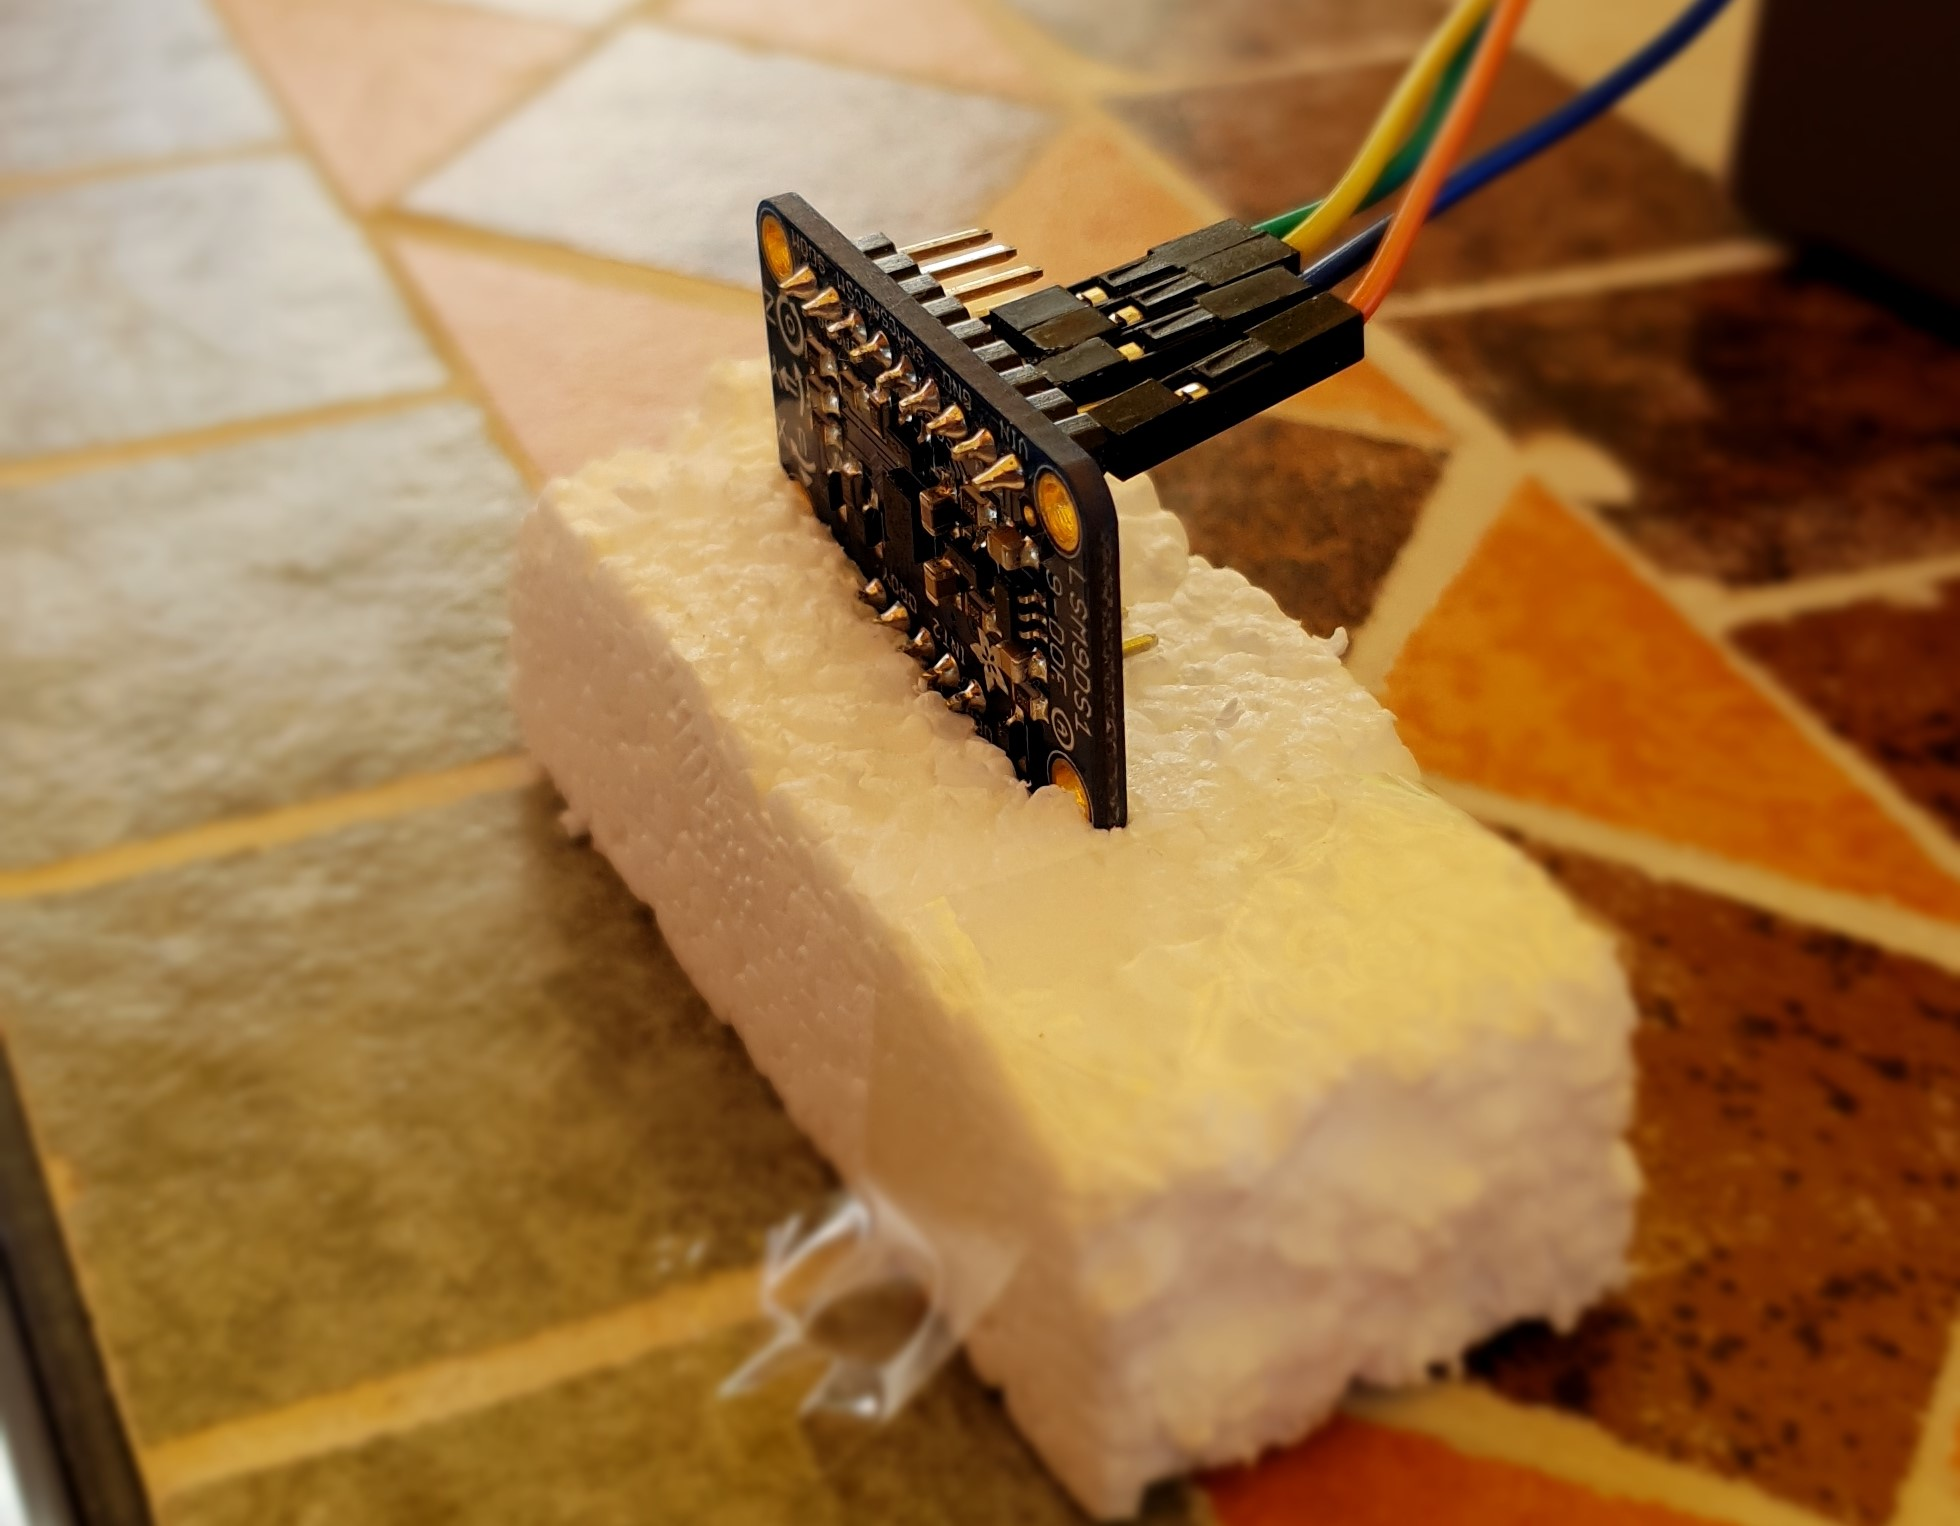
\includegraphics[width=40mm]{analisi/x.jpg}}
	\subfigure[]{\label{fig:y}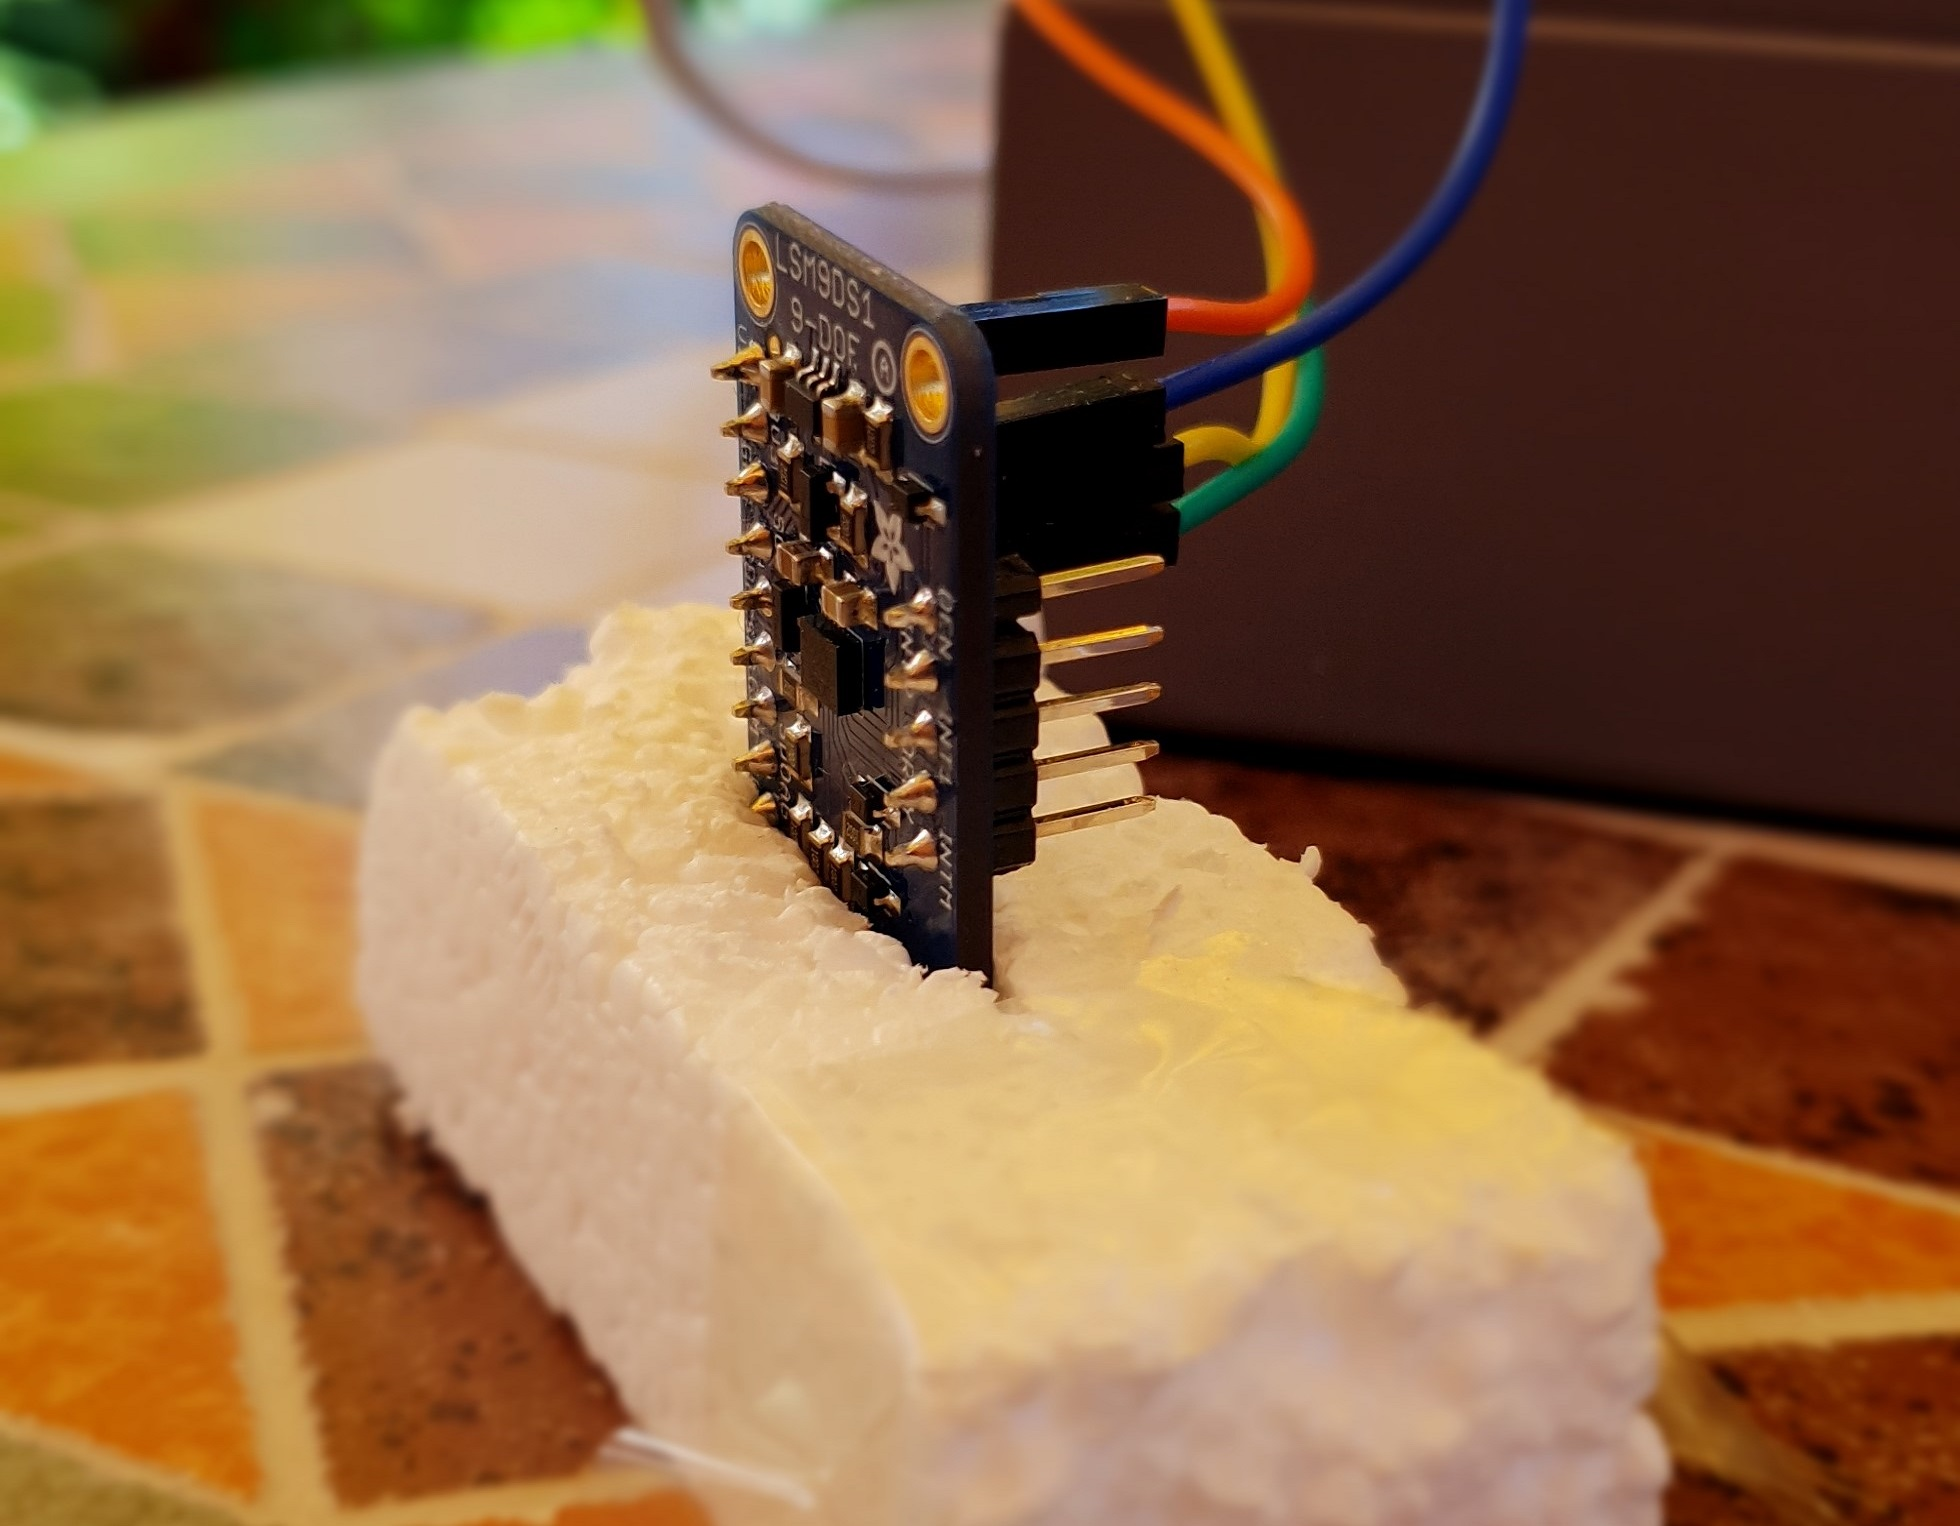
\includegraphics[width=40mm]{analisi/y.jpg}}
	\subfigure[]{\label{fig:z}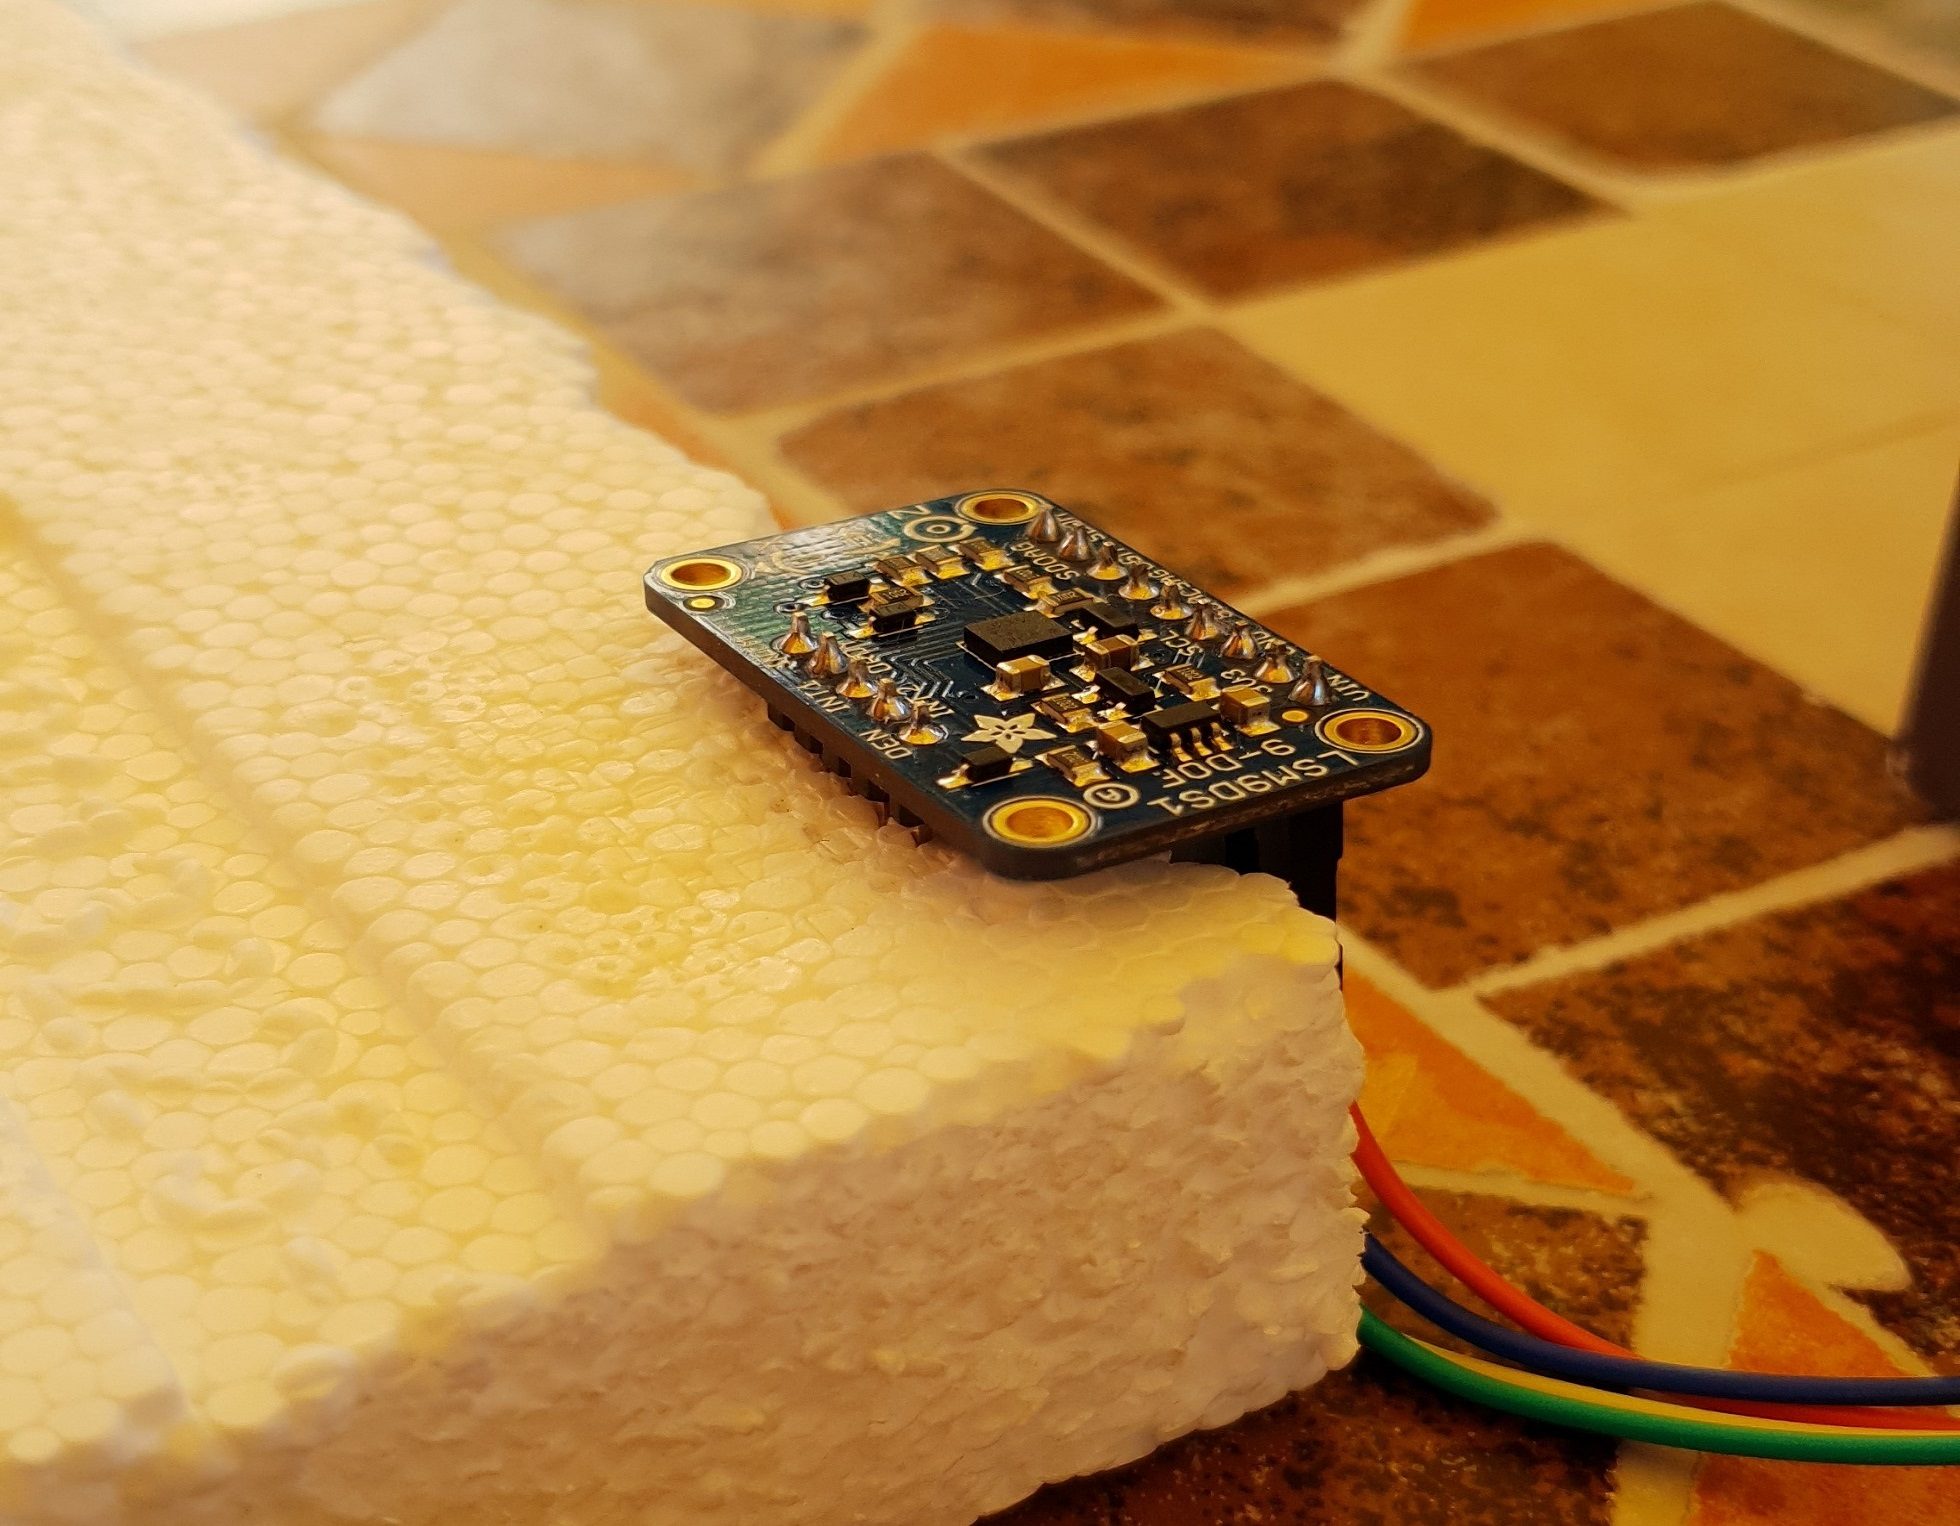
\includegraphics[width=40mm]{analisi/z.jpg}}
	\caption{in \ref{fig:x} l'IMU posto parallelamente all'asse \textit{X}, in \ref{fig:y} l'IMU posto parallelamente all'asse \textit{Y} e infine in \ref{fig:z} l'IMU posto parallelamente all'asse \textit{Z}}
\end{figure}
Quindi per ogni lettura si è determinata la norma euclidea, dalla quale banalmente si ottiene il modulo dello zero-g offset sottraendo 1. Tale valore è da considerarsi come modulo e non sui singoli assi in quanto il dispositivo potrebbe non essere stato posizionato perfettamente parallelo all'asse in questione. In Fig.\ref{fig:andamentizero-g} vengono mostrati i valori degli zero-offset per i campioni catturati nei primi 7 secondi per ognuno dei tre assi:

\begin{figure}[H]
	\centering    
	\subfigure[]{\label{fig:zgx}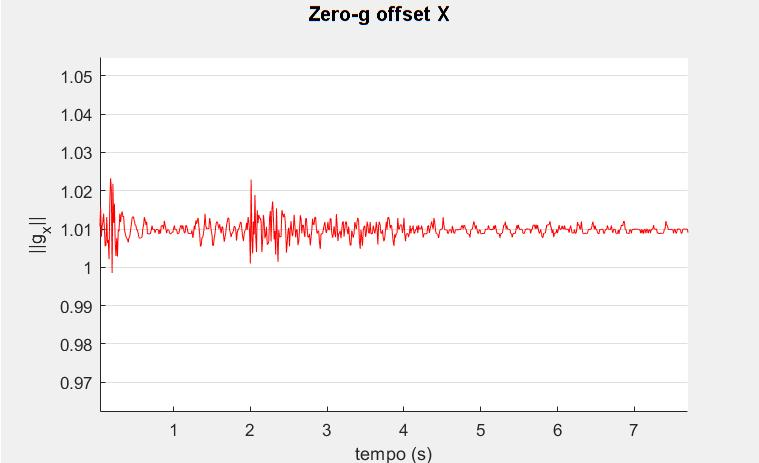
\includegraphics[width=80mm]{analisi/x-offset.jpg}}
	\subfigure[]{\label{fig:zgy}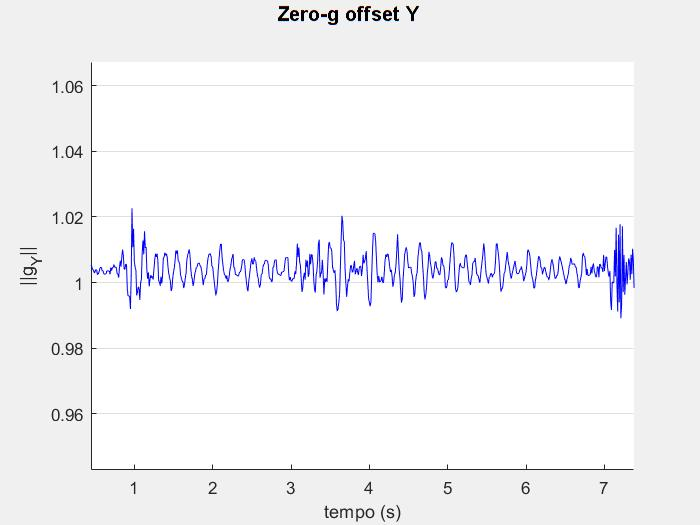
\includegraphics[width=80mm]{analisi/y-offset.jpg}}
	\subfigure[]{\label{fig:zgz}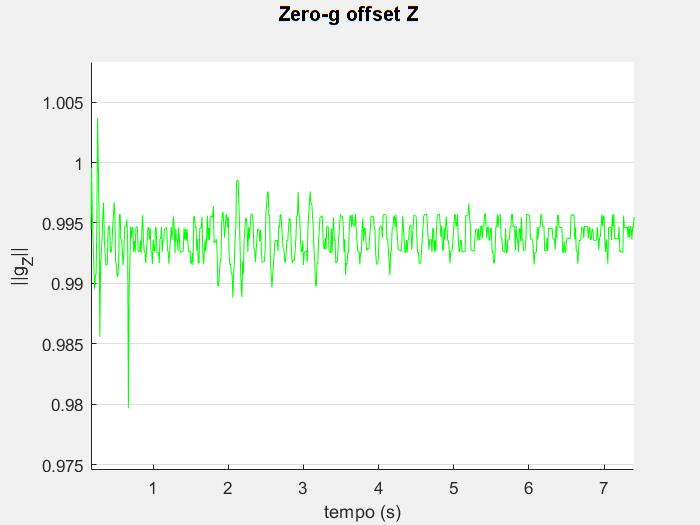
\includegraphics[width=80mm]{analisi/z-offset.jpg}}
	\label{fig:andamentizero-g}
	\caption{valori degli zero-g offset calcolati rispettivamente sull'asse X \ref{fig:zgx}, sull'asse Y  \ref{fig:zgy} e sull'asse \ref{fig:zgz}}
\end{figure}

Nella Tab.\ref{tab:zero-g} si riportano i valori di \textit{Media, Max} e le percentuali di occorrenze dei valori compresi nell'intervallo (0,1) e maggiori di 1.

\begin{table}[H]
	\centering
	\label{tab:zero-g}
	\begin{tabular}{|c|c|c|c|c|}
		\hline
		\textbf{Asse} & \multicolumn{1}{l|}{\textbf{Media (G)}} & \multicolumn{1}{l|}{\textbf{Max (G)}} & \textbf{ val>1} & \textbf{ 0<val>1} \\ \hline
			x             & 1,0096                                  & 1,0233                                & 99               & 1                  \\ \hline
			y             & 1,0036                                  & 1,0266                                & 99               & 1                  \\ \hline
			z             & 0,9936                                  & 1,0037                                & 0,02             & 99,08              \\ \hline
		\end{tabular}
	\caption{Media, Max e percentuali di occorrenze dei valori compresi nell'intervallo (0,1) e maggiori di 1 dei dati mostrati in Fig.\ref{fig:zgx} }
	\end{table}


\subsection{Stima dello zero-rate offset}
\label{zero_rate}
Per stimare lo zero-rate offset si è posto immobile l'IMU (come in Fig.\ref{fig:zero-g}) e si sono raccolti i dati letti dal giroscopio per un totale di due minuti. I valori ottenuti, per ognuno dei tre assi, sono mostrati in Fig.\ref{fig:zero-rate}:
\begin{figure}[H]  
	\centering 
	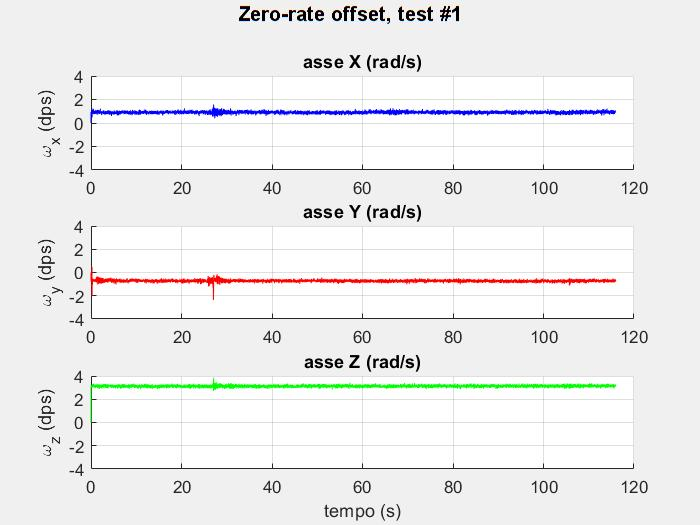
\includegraphics[scale=0.6]{analisi/zero-rate.jpg}
	\caption{valori degli zero-rate offset per i campioni catturati in 2 minuti rispettivamente sull'asse X, Y e Z.}
	\label{fig:zero-rate}
\end{figure}
Dai valori mostrati in Fig.\ref{fig:zero-rate} si evince facilmente la presenza di un offset significativo sull'asse Z da cui ne consegue che, pur rimanendo immobile il giroscopio ha \textit{"la sensazione"} di essere ruotato intorno all'asse in questione con una velocità angolare significativa.\\
Nella Tab.\ref{tab:zero-rate} si riportano invece i valori di \textit{media} e \textit{varianza} per i campioni mostrati in Fig.\ref{fig:zero-rate}:
\begin{table}[H]
	\centering
	\label{tab:zero-rate}
	\begin{tabular}{|c|c|c|l}
		\cline{1-3}
		\textbf{Asse} & \multicolumn{1}{l|}{\textbf{Media (dps)}} & \multicolumn{1}{l|}{\textbf{Varianza}} &  \\ \cline{1-3}
		x             & 0,9055                                    & 0,0079                                 &  \\ \cline{1-3}
		y             & -0,7203                                   & 0,0091                                 &  \\ \cline{1-3}
		z             & 3,1291                                    & 0,0064                                 &  \\ \cline{1-3}
	\end{tabular}
	\caption{Media e varianza per i valori di zero-rate offset mostrati in Fig.\ref{fig:zero-rate}}
\end{table}
\subsection{Conclusioni stima dello zero-offset}
L'analisi appena effettuata ha mostrato come i dati grezzi provenienti dall'unità di misura inerziale (Cap.\ref{tecnologie}) siano affetti dallo zero-offset.\\
L'accelerometro non risulta subire molto questo fenomeno, infatti i valori medi dei moduli del vettore gravitazionale si discostano al più dello 0,96\% (\ref{tab:zero-g}) sull'asse delle \textit{X} e il valore massimo si ha in corrispondenza dell'asse \textit{Y} che supera il valore ideale di $0,0266 G$. \\
Ben diversa è la situazione dello zero-rate offset che risulta essere molto significativo sopratutto sull'asse \textit{Z} dove si ha una media di $3,1291 dps$. I valori di varianza bassi sottolineano come tale errore sia relativamente constante nel tempo fornendo quindi un punto di partenza per una sua modellizzazione.\\
A valle di queste considerazioni si vuole evidenziare come l'uso dei dati grezzi provenienti dall'IMU per un'elaborazione che permetta la stima dell'assetto, debba essere preceduto da un'attività di compensazione di tali offset. Compensazione che può, in alcuni casi, trasformarsi in un vero e proprio lavoro di caratterizzazione e modellizzazione dell'errore all'interno dell'algoritmo di elaborazione. 





\section{Analisi qualitativa dell'assetto stimato}
\label{analisiQualitativa}
Quest'analisi ha lo scopo di verificare la correttezza dell'algoritmo di \textit{sensor fusion} implementato (sez.\ref{sensor_fusion}) e della libreria \textit{MotionFX} \cite{motion}. In particolare si vuole confrontare la stima dello \textit{yaw} (sez.\ref{angoliEulero}) a seguito di varie sollecitazioni. Questo perché la stima dell'imbardata è, attualmente, quella più utile per  identificare gli angoli assunti dall'operatore nel tragitto tra un nodo e l'altro (cap.\ref{descrizioeDelLavoro}).\\
Per fare questo si è realizzato un "sistema ausiliario" ad hoc in grado di ruotare l'unità di misura inerziale ripetutamente e di un certo angolo. Tale sistema è composto da:
\begin{itemize}
	\item Un Arduino duemilanove
	\item Un servo motore MG995
\end{itemize}
Ed è rappresentato dalla seguente figura:
\begin{figure}[H]  
	\centering 
	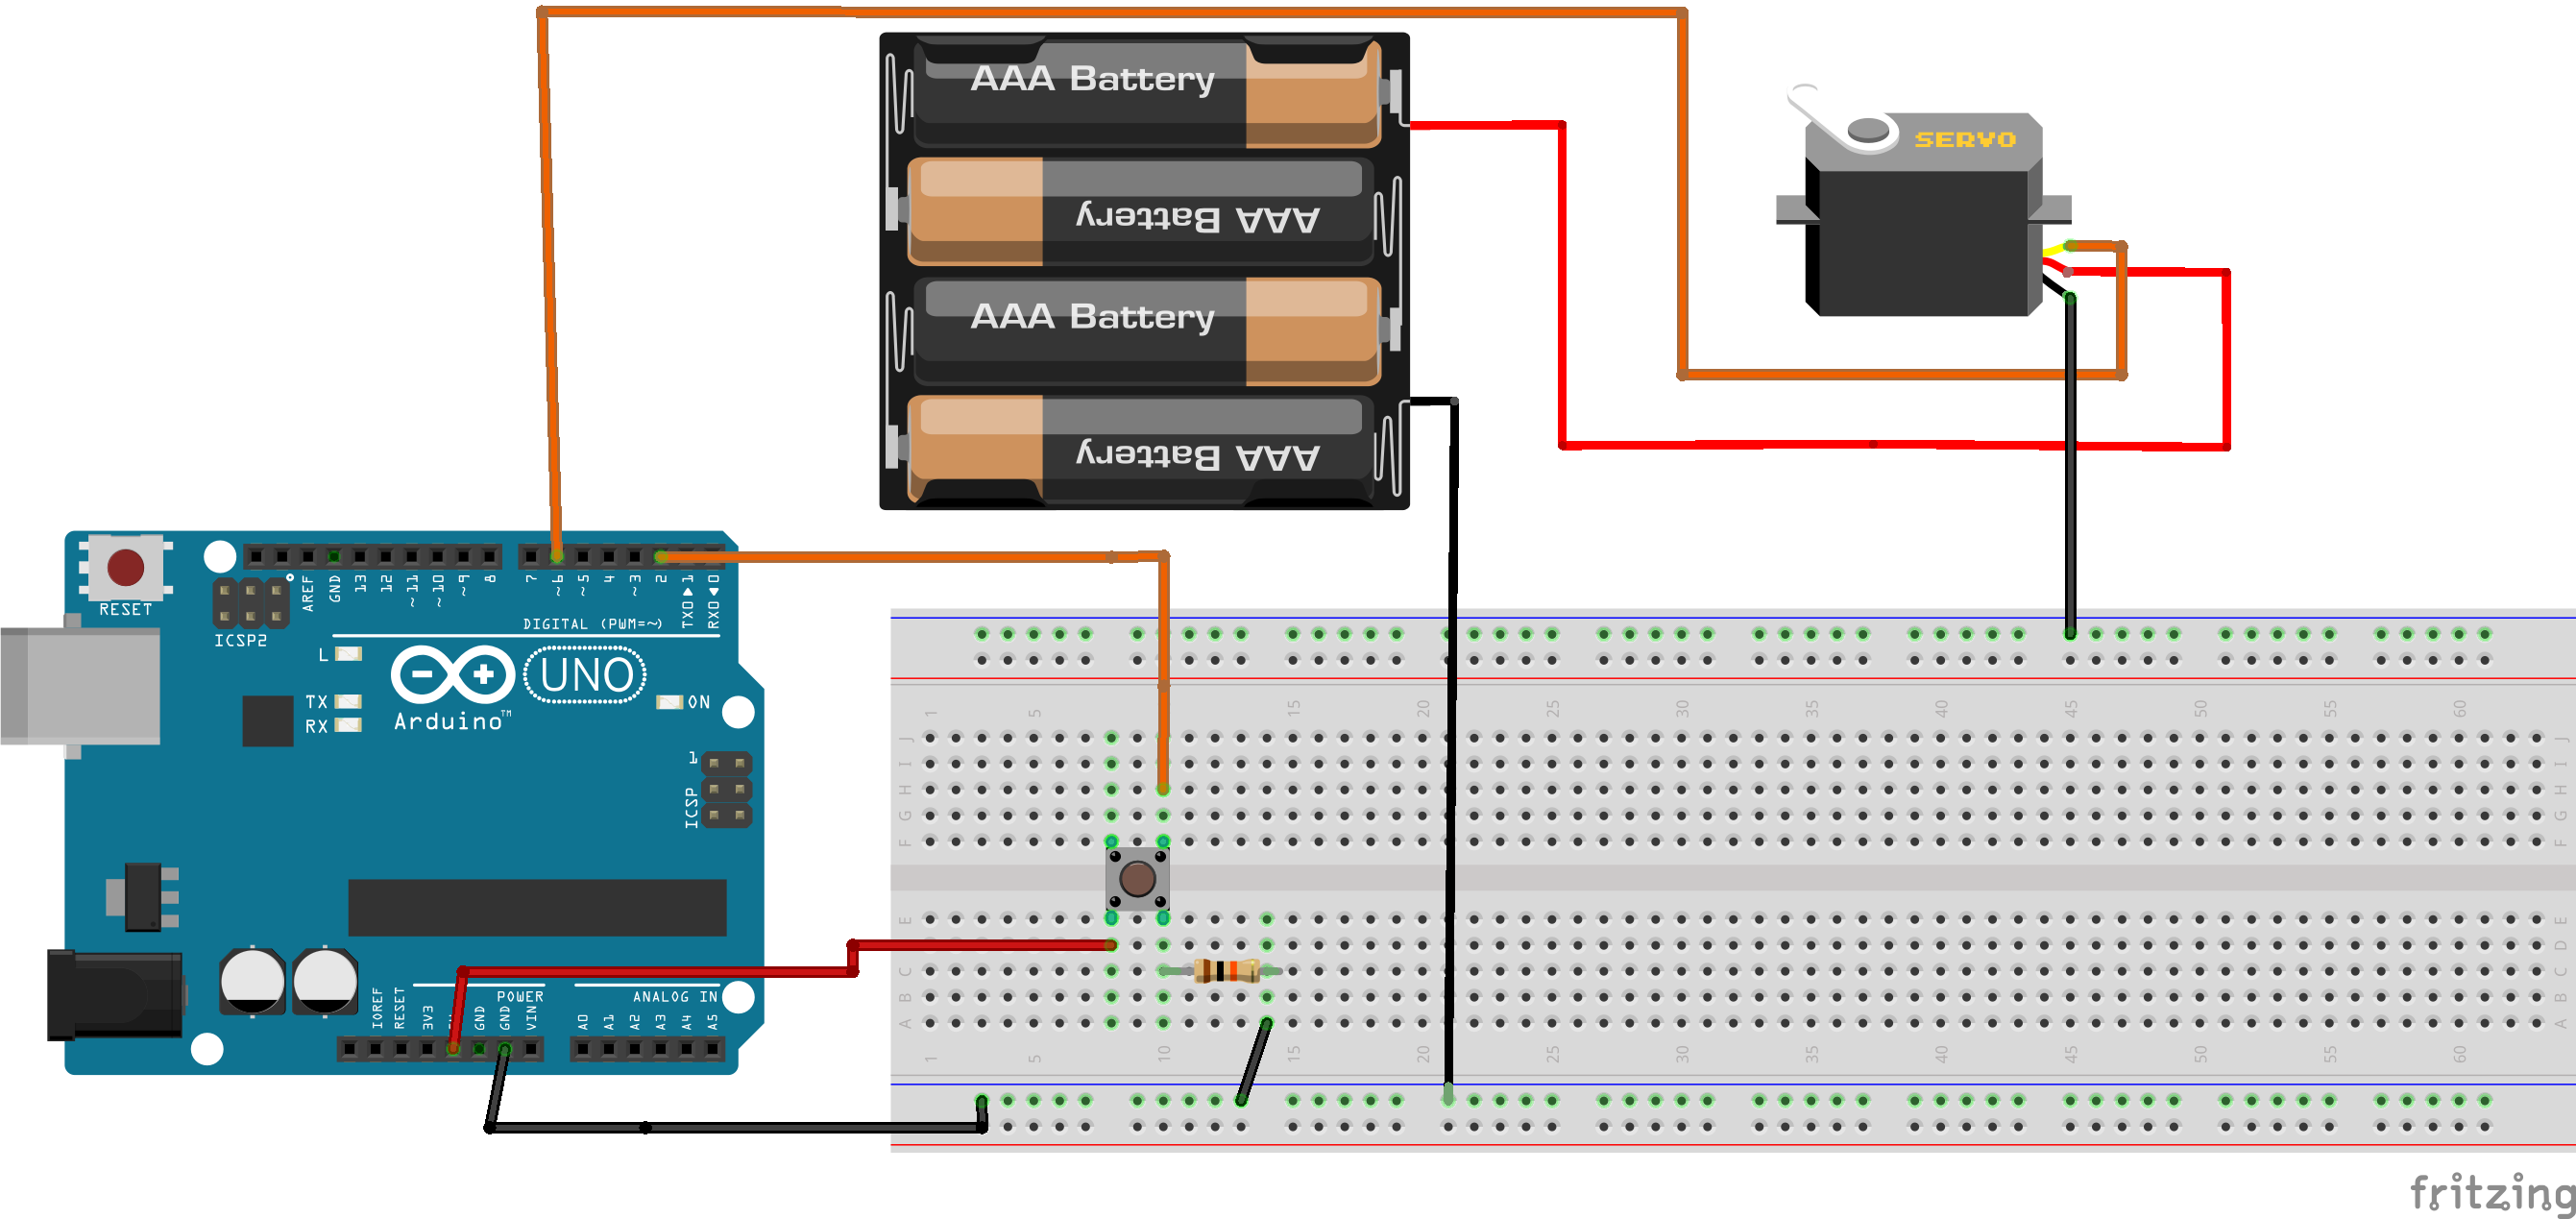
\includegraphics[scale=0.5]{analisi/servo.png}
	\caption{Schema hardware del sistema ausiliario realizzato per eseguire l'analisi qualitativa}
	\label{fig:arduino}
\end{figure}
Alla pressione del bottone mostrato in Fig.\ref{fig:arduino}, il codice all'interno di Arduino (App.\ref{app:scriptArduino}) manda un impulso al servo motore grazie al quale il servo ruota di $90^{\circ}$. Quindi Arduino attende 500 ms prima di inviare un'ulteriore segnale affinché il servo torni alla posizione iniziale. Questa procedura viene ripetuta dieci volte aspettando 1 secondo tra le prime cinque rotazioni di $\pm 90^{\circ}$ e le ultime. Il modulo App elabora i dati grezzi letti dal modulo Microcontrollore (sez.\ref{impl_hardware}) a seguito di questi movimenti e applica l'algoritmo di \textit{Sensor fusion} implementato. \\
Le stime dello \textit{yaw} ottenute dai due moduli, a partire dagli stessi dati grezzi, sono mostrate dalle seguente figura:
\begin{sidewaysfigure}[htbp]
	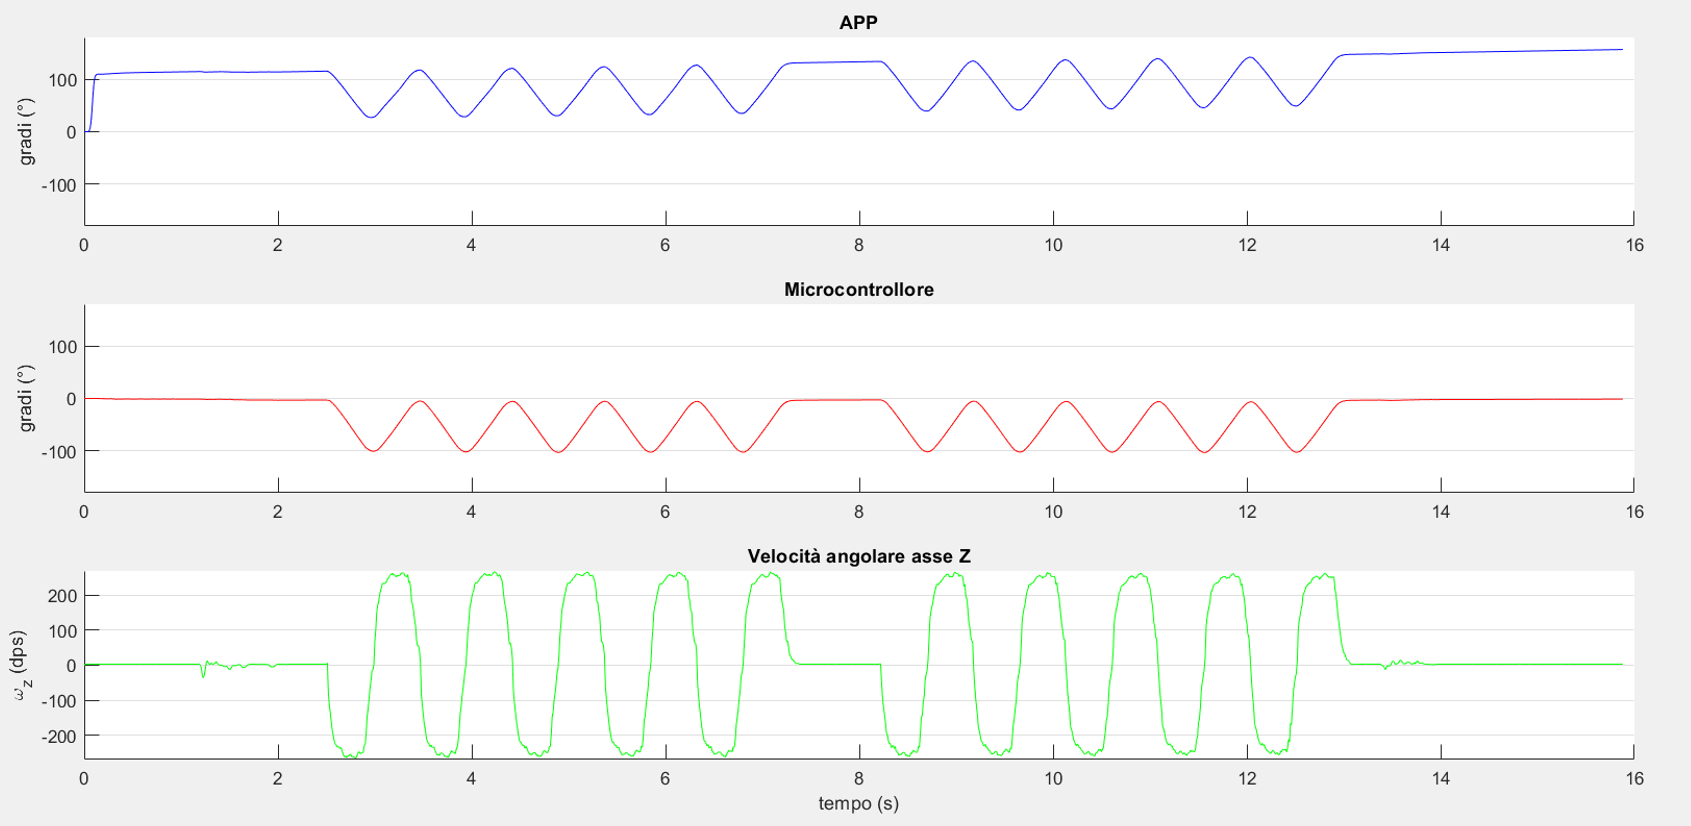
\includegraphics[width=\textwidth]{analisi/analisiQualitativa.png}
	\caption{Risultati analisi qualitativa}
	\label{fig:analisiQualitativa}
\end{sidewaysfigure}
\newpage
Come si può notare dalla Fig.\ref{fig:analisiQualitativa}, la risposta generale dei due algoritmi è buona. Infatti entrambi rispondono correttamente ai movimenti rotatori effettuati intorno all'asse $Z$ dell'IMU facendo oscillare lo \textit{yaw} di $\pm 90^{\circ}$ rispetto all'angolo di partenza ( da notare che per il modulo APP è circa  $ 110^{\circ}$ mentre per il micro è  $0^{\circ}$ ).\\
Tuttavia si nota facilmente come la stima da parte del modulo APP diverga sempre più, muovendo verso l'alto il range dei valori picco-picco. Tale variazione è costante e rappresentata dalla seguente figura:
\begin{figure}[H]  
	\centering 
	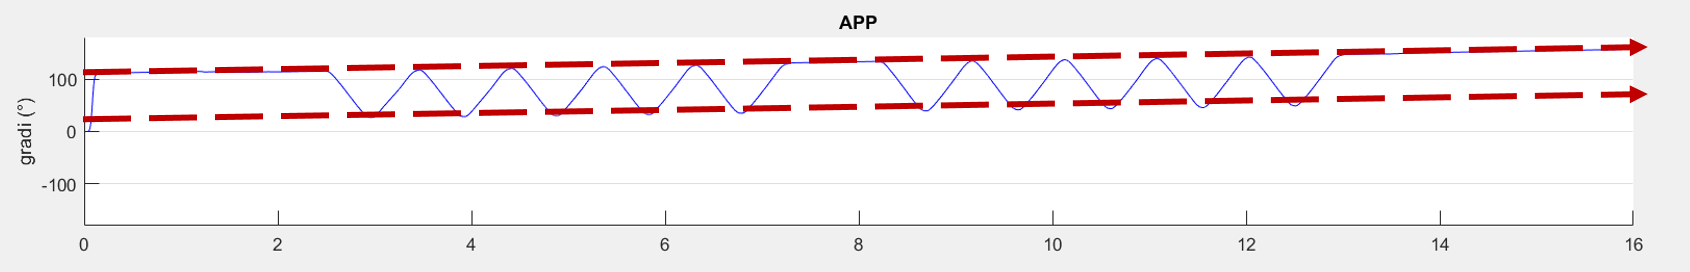
\includegraphics[scale=0.35]{analisi/analisiQualitativaApp.png}
	\caption{Retta di divergenza della stima dello \textit{yaw} eseguita dal modulo APP.}
	\label{fig:analisiQualitativaApp}
\end{figure}
A partire da un angolo stimato di $ 110^{\circ}$ lo \textit{yaw} dopo dieci rotazioni di $\pm 90^{\circ}$ effettuate in $\approx 15 sec$ lo \textit{yaw} finale risulta essere  $ 157^{\circ}$. Da tali valori si calcola facilmente che il coefficiente angolare delle rette di divergenza mostrate in Fig.\ref{fig:analisiQualitativaApp} è di $3,13$. Questo risultato è coerente con quanto emerso nell'analisi dello zero-rate (sez.\ref{zero_rate}), ovvero che lungo l'asse z si ha un \textit{drift} di valore medio pari a $\approx 3,12 dps$.\\
Alla luce di questa analisi è facile capire come l'algoritmo di \textit{Sensor fusion} (sez.\ref{sensor_fusion}) implementato e utilizzato dal modulo APP non tenga conto di questo fenomeno, cosa che avviene invece all'interno della libreria \textit{MotionFX} utilizzata dal modulo Microcontrollore poiché i valori picco-picco restano confinati all'interno dell'intervallo $[0^{\circ},-90^{\circ}]$ come mostrato dalla Fig.\ref{fig:analisiQualitativa}.





\chapter{Conclusioni e prospettive future}
\label{conclusioni}
A seguito dell'analisi qualitativa effettuata (sez.\ref{analisiQualitativa}), l'azienda presso la quale è stata svolta questa tesi
 ha ritenuto il lavoro fatto più che soddisfacente riconoscendo di aver acquisito tramite esso un sistema in grado di stimare l'assetto di un operatore con un margine di errore non significativo ai fini dell'applicazione e di aver contribuito ad arricchire il know-how aziendale riguardante la stima dell'assetto.\\
A partire dal lavoro di questa tesi vi sono molte prospettive, alcune delle quali verranno affrontate da proposte di tesi future:
\begin{itemize}
	\item Ottimizzazione dell'operazione di lettura delle misure dall'unità di misura inerziale tramite I2C.
	\item Caratterizzazione degli zero-offset e loro compensazione nell'algoritmo di \textit{Sensor Fusion} implementato.
	\item Identificazione della soluzione ottima per la realizzazione del modulo App.
\end{itemize}

Una volta realizzato interamente il sistema ideato e descritto nel capitolo \ref{descrizioeDelLavoro}, si avrà uno strumento innovativo in grado di fornire un aiuto significativo agli operatori che si trovano ad affrontare situazioni d'emergenza di questo tipo; contribuendo a salvare più vite umane.
\newpage

\pagenumbering{roman}
\appendix

	\chapter{Rotazioni nello spazio}






%\chapter*{Ringraziamenti}
\markboth{Ringraziamenti}{Ringraziamenti}
\addcontentsline{toc}{chapter}{Ringraziamenti}
\thispagestyle{empty}

Desidero ringranziare sentitamente il prof. Giovanni De Gasperis per i preziosi consigli e il tempo dedicatomi. Inoltre desidero ringraziare la prof.ssa Laura Tarantino per avermi proposto questo affascinante lavoro e per i suoi utili insegnamenti, i quali hanno contribuito significativamente alla mia attuale formazione professionale come ingegnere.\\
Inoltre desidero ringraziare i miei amici e la mia compagna per avermi supportato durante tutto il mio percorso. Infine dedico questo e tutti i miei futuri successi alla mia famiglia, il mio carburante, la mia unica variabile globale.


% BEGIN Bibliografia
\begin{thebibliography}{99}
\addcontentsline{toc}{chapter}{Bibliografia}

\bibitem{context}
Towards a Better Understanding of Context and Context-Awareness
\author{Anind K. Dey, Gregory D. Abowd}
\url{ftp://ftp.cc.gatech.edu/pub/gvu/tr/1999/99-22.pdf}

\bibitem{gps}
Sistema di posizionamento globale
\url{https://it.wikipedia.org/wiki/Sistema_di_posizionamento_globale#cite_note-1}


\bibitem{IPS}
Indoor positioning system
\url{https://en.wikipedia.org/wiki/Indoor_positioning_system}

\bibitem{IPS2}
Progettazione e realizzazione di un Indoor Positioning System basato su geomagnetismo e sensor fusion
\url{http://amslaurea.unibo.it/12840/1/federico_torsello_tesi.pdf}

\bibitem{alg1}
Luca Pappalardo, "Localizzazione - Problema, Tecniche, Algoritmi - Reti mobili:
Ad Hoc e di sensori", 2011,
\url{http://didawiki.di.unipi.it/lib/exe/fetch.php/rhs/localizzazione.pdf}

\bibitem{alg2}
Cuccado, De Franceschi, Fauri, Sartor, "Analisi di algoritmi di autolocalizzazione
per reti di sensori wireless", 2007,
\url{https://art.torvergata.it/retrieve/handle/2108/773/6945/Paolo-Sperandio-Tesi-PhD.pdf}

\bibitem{indoorThesis}
An adaptive indoor positioning system based on Bluetooth Low Energy RSSI
\author{Nicola Cinefra}
\url{https://www.politesi.polimi.it/bitstream/10589/92284/3/NicolaCinefra770910TesiDefinitiva.pdf}

\bibitem{market}
Harrop P, Raghu D. Mobile Phone Indoor Positioning Systems (IPS) and Real Time
Locating Systems (RTLS) 2014-2024. Forecasts, Players, Opportunities. IDTechEx



\bibitem{rssi}
Ugur Bekcibasi, "Increasing RSSI Localization Accuracy with Distance Reference
Anchor in Wireless Sensor Networks", 2014,
\url{http://www.uni-obuda.hu/journal/Bekcibasi_Tenruh_54.pdf}

\bibitem{toaProblem}
Mak LC, Furukawa T. A ToA-based Approach to NLOS Localization Usiong Low-Frequency Sound. ACRA2006 (Auckland, New Zealand); 2006


\bibitem{aoa}
A Simple Technique for angle of arrival measurement
\url{https://www.researchgate.net/publication/4368716_A_Simple_Technique_for_angle_of_arrival_measurement}

\bibitem{triangolazione}
Generalized Geometric Triangulation Algorithm for Mobile Robot
Absolute Self-Localization 
\url{https://pdfs.semanticscholar.org/dee6/fb124433cac10744afd9502b165ffdecb202.pdf}

\bibitem{sensorfusion}
Sensor fusion
\url{https://en.wikipedia.org/wiki/Sensor_fusion}

\bibitem{mems}
Jeroen Hol "Sensor Fusion and Calibration of
Inertial Sensors, Vision,
Ultra-Wideband and GPS"
\url{https://www.xsens.com/wp-content/uploads/2014/pdf/Hol2011%20-%20Dissertation.pdf}

\bibitem{principimems}
Janusz Bryzek "Principles of MEMS"
\url{https://www.wiley.com/legacy/wileychi/hbmsd/pdfs/mm573.pdf}


\bibitem{acc}
MEMS Accelerometer
\url{http://www.instrumentationtoday.com/mems-accelerometer/2011/08/}


\bibitem{gyromodel}
H. Titterton and J. L. Weston. Strapdown inertial navigation technology. IEE
radar, sonar, navigation and avionics series. Peter Peregrinus Ltd., Stevenage,
UK, 1997. ISBN 0863413587.

\bibitem{corolois}
Forza di Coriolis, Wikipedia
\url{https://it.wikipedia.org/wiki/Forza_di_Coriolis}

\bibitem{gyroMems}
The Development of Micromachined Gyroscope Structure and
Circuitry Technology, Dunzhu Xia, Cheng Yu and Lun Kong

\bibitem{assetto}
TECNICHE DI STIMA E CONTROLLO DI ASSETTO DI
SATELLITI. Andrea Fagiani. 
\url{http://control.disp.uniroma2.it/carnevale/archivio/Tesi/andreafagianiM/tesi.pdf}




\bibitem{trackingThesis}
Advanced algorithms and architectures for MEMS inertial sensor platforms 
in orientation tracking and in fall detection applications. Simone Sabatelli.
Università di Pisa.

\bibitem{motion}
MotionFX middleware library in X-CUBE-MEMS1 software
expansion for STM32Cube.\\
\url{http://www.st.com/content/ccc/resource/technical/document/user_manual/group0/31/0e/66/39/cb/f7/4e/cd/DM00394369/files/DM00394369.pdf/jcr:content/translations/en.DM00394369.pdf}


\end{thebibliography}




% END Bibliografia


\end{document}